\documentclass[a4paper,12pt]{article}

% --- PACKAGES ---
% =============================
% --- ENCODAGE & TYPOGRAPHIE ---
% =============================
\usepackage[utf8]{inputenc}
\usepackage[T1]{fontenc}
\usepackage{lmodern}
\usepackage{microtype}
\usepackage{setspace}
\usepackage{indentfirst}
\usepackage{ragged2e}
\usepackage{parskip}

% Guillemets francais « » : commandes \og ... \fg sans charger babel
% (babel-french doublerait les espaces des « ~: » deja presents dans le texte)
\providecommand{\og}{\guillemotleft\,}
\providecommand{\fg}{\,\guillemotright}

\usepackage{siunitx}
\sisetup{detect-all, output-decimal-marker={,}}

% =============================
% --- MISE EN PAGE ---
% =============================
\usepackage[margin=2.5cm]{geometry}
\usepackage{fancyhdr}
\usepackage{titlesec}
\usepackage{needspace}

% =============================
% --- COULEURS & GRAPHISME ---
% =============================
\usepackage[table]{xcolor}
\usepackage{transparent}
\usepackage{tikz}
\usetikzlibrary{shadows}

% =============================
% --- IMAGES / PDF / WRAP ---
% =============================
\usepackage{graphicx}
\usepackage{wrapfig}
\usepackage{pdfpages}
\usepackage[absolute,overlay]{textpos}

% =============================
% --- POLICE PAR DÉFAUT ---
% =============================
\usepackage{helvet}
\renewcommand{\familydefault}{\sfdefault}

% =============================
% --- TABLEAUX ET LISTINGS ---
% =============================
\usepackage{tabularx}
\usepackage{array}
\usepackage{booktabs}
\usepackage{listings}
\newcolumntype{C}{>{\centering\arraybackslash}X}
\renewcommand{\arraystretch}{1.4}

% =============================
% --- HYPERREF & URL ---
% =============================
\usepackage{hyperref}
\usepackage{url}
\usepackage{xurl}

% =============================
% --- ALGORITHMES ---
% =============================
\usepackage{algorithm}
\usepackage{algpseudocode}

% =============================
% --- INFORMATIQUE ---
% =============================
\usepackage{minted}
\usemintedstyle{lovelace}

% =============================
% --- MATH ---
% =============================
\usepackage{amsmath}
\usepackage{amssymb}
\usepackage{amsfonts}

% =============================
% --- ANNEXES & CITATIONS ---
% =============================
\usepackage[toc]{appendix}
\usepackage{csquotes}
\usepackage{tcolorbox}

% =============================
% --- PIFONT (CHECKS ICONES) ---
% =============================
\usepackage{pifont}
\newcommand{\good}{\ding{51}}
\newcommand{\bad}{\ding{55}}

% =============================
% --- WARNINGS LaTeX ---
% =============================
\hfuzz=2pt
\hbadness=10000

% =============================
\usepackage[framemethod=tikz]{mdframed}

% --- STYLES ---
% --- STYLES ---

% ========================
%       INDENTATION
% ========================
\setlength{\parindent}{1.5em}      % Indentation automatique des paragraphes

% ========================
%         COULEURS
% ========================
\definecolor{title1}{RGB}{32, 94, 153} % Bleu foncé (titres de sections)
\definecolor{title2}{RGB}{75, 147, 215} % Bleu clair (titres de sous-sections)
\definecolor{footer}{RGB}{75, 147, 215}

% ========================
%   FORMATTAGE DES TITRES
% ========================
\titleformat{\section}
  {\color{title1}\normalfont\Large\bfseries\fontfamily{cmss}}
  {\color{title1}\thesection}{1em}
  {\MakeUppercase}
  [\noindent\color{black}\rule{\textwidth}{0.5pt}]

\titleformat{\subsection}
  {\color{title2}\normalfont\large\bfseries\fontfamily{cmss}}
  {\color{title2}\thesubsection}{1em}
  {\MakeUppercase}
  [\noindent\color{black}\rule{\textwidth}{0.4pt}]

% ========================
%   PERSONNALISATION LISTES
% ========================
\renewcommand{\contentsname}{Table des Matières}
\renewcommand{\listfigurename}{Table des Figures}
\renewcommand{\appendixname}{Annexe}

% ========================
%    STYLE DES PAGES
% ========================
\pagestyle{empty} % Pas d'en-tête ni pied de page par défaut

% ========================
% POSITIONNEMENT TEXTBLOCK
% ========================
\setlength{\TPHorizModule}{1cm}
\setlength{\TPVertModule}{1cm}

% ========================
\hypersetup{
    colorlinks=true,
    linkcolor=black,
    urlcolor=blue,
    citecolor=blue
}

% ========================
%     STYLE DES CAPTIONS
% ========================
\newmdenv[
  topline=false,
  rightline=false,
  bottomline=false,      % Active la ligne du bas
  linewidth=2pt,         % Épaisseur de la barre verticale
  linecolor=black,       % Couleur de la barre verticale
  innerleftmargin=10pt   % Optionnel : espace après le bloc
  innertopmargin=15pt
]{captionbox}


% Configuration de la coloration syntaxique pour JavaScript
\definecolor{codegreen}{rgb}{0,0.6,0}
\definecolor{codegray}{rgb}{0.5,0.5,0.5}
\definecolor{codepurple}{rgb}{0.58,0,0.82}
\definecolor{backcolour}{rgb}{0.95,0.95,0.92}

\lstdefinestyle{jsstyle}{
    backgroundcolor=\color{backcolour},
    commentstyle=\color{codegreen},
    keywordstyle=\color{magenta},
    numberstyle=\tiny\color{codegray},
    stringstyle=\color{codepurple},
    basicstyle=\ttfamily\footnotesize,
    breakatwhitespace=false,
    breaklines=true,
    captionpos=b,
    keepspaces=true,
    numbers=left,
    numbersep=5pt,
    showspaces=false,
    showstringspaces=false,
    showtabs=false,
    tabsize=2,
    language=Java
}

\usetikzlibrary{arrows.meta,positioning,calc,shapes.geometric,decorations.text}
\usepackage{fontawesome5}
\usepackage{adjustbox}
\usepackage{xurl}
% Couleurs du schéma d'architecture
\definecolor{archbleu}{HTML}{1F4E79}
\definecolor{archgris}{HTML}{404040}
\definecolor{archorange}{HTML}{F28C28}
\definecolor{archvert}{HTML}{21A366}
\definecolor{archjaune}{HTML}{F2C811}
\definecolor{archrouge}{HTML}{E8505B}
\usepackage{pdflscape}
% Tableaux du modèle de données : bordures bleu clair, en-tête bleuté, texte en 9 pt
\definecolor{tabbordure}{HTML}{8EAADB}
\definecolor{tabentete}{HTML}{D9E2F3}
\newenvironment{tableau}[1]{\par\vspace{6pt}\noindent\fontsize{9}{11}\selectfont
  \setlength{\tabcolsep}{4pt}\renewcommand{\arraystretch}{1.15}%
  \arrayrulecolor{tabbordure}%
  \begin{tabular}{#1}\hline}{\end{tabular}\arrayrulecolor{black}\par\vspace{6pt}}
% Séparateur entre définitions : jamais en haut ni en bas de page
% (filet en \cleaders, supprimé par TeX s'il tombe sur une coupure de page)
\newcommand{\separateur}{\par\needspace{8\baselineskip}\vskip0.4cm%
  \cleaders\hbox to\linewidth{\hss\rule{5cm}{0.4pt}\hss}\vskip0.5pt\nobreak}
\newcommand{\source}[1]{\par\nobreak\vspace{-0.2cm}\nobreak{\centering\footnotesize\textit{Source~: #1}\par}}
\newcommand{\legende}[1]{\par\nobreak\vspace{0.25cm}\nobreak{\centering\footnotesize\textit{#1}\par}}
% Capture d'un job Talend (contents/img/jobs/<nom>.png), cadre provisoire si l'image manque
\newcounter{figjob}\setcounter{figjob}{3}
\newcommand{\capturejob}[2]{\stepcounter{figjob}%
  \begin{center}\IfFileExists{contents/img/jobs/#1.png}%
    {\adjustbox{max width=\linewidth,max height=8cm}{\includegraphics{contents/img/jobs/#1.png}}}%
    {\fbox{\parbox[c][2.2cm][c]{0.8\linewidth}{\centering\footnotesize\textit{Capture à venir}}}}%
  \legende{Figure~\thefigjob{} -- #2}\end{center}}
% Fiche d'un job : nom de l'image, titre, source, traitement, valeurs nulles et doublons
% Une fiche n'est jamais coupée entre deux pages : si elle ne tient pas, elle passe entière à la page suivante.
\newcommand{\fichejob}[5]{\par\vspace{0.6cm}\noindent\begin{minipage}{\linewidth}
  \subsubsection*{#2}
  \capturejob{#1}{Job #2}
  \noindent\textbf{Source~:} #3\par\vspace{0.1cm}
  \noindent\textbf{Traitement~:} #4\par\vspace{0.1cm}
  \noindent\textbf{Valeurs nulles et doublons~:} #5\par
  \end{minipage}\par}

% --- RÈGLES DE MISE EN PAGE ---
% Paragraphes, listes et cases de tableau jamais coupés entre deux pages,
% pas de ligne seule en haut ou en bas de page
\interlinepenalty=10000
\clubpenalty=10000
\widowpenalty=10000
\displaywidowpenalty=10000
\makeatletter
\@itempenalty=10000
% Une liste reste attachée à la phrase qui l'introduit
\AtBeginEnvironment{itemize}{\@beginparpenalty=10000}
\AtBeginEnvironment{enumerate}{\@beginparpenalty=10000}
\makeatother
% Un titre part à la page suivante s'il ne reste pas la place d'un vrai bloc.
% \needspace redéfini sans son \penalty-100, qui faisait préférer une coupure
% avant chaque titre et laissait de grands blancs en bas de page ;
% pas de coupure forcée si la page est déjà pleine (elle se coupera d'elle-même)
\makeatletter
\renewcommand{\needspace}[1]{\par\begingroup\setlength{\dimen@}{#1}%
  \dimen@ii\pagegoal\advance\dimen@ii-\pagetotal
  \ifdim\dimen@>\dimen@ii\ifdim\dimen@ii>\z@\vfil\break\fi\fi\endgroup}
\makeatother
\usepackage{etoolbox}
\pretocmd{\section}{\needspace{14\baselineskip}}{}{}
\pretocmd{\subsection}{\needspace{10\baselineskip}}{}{}
\pretocmd{\subsubsection}{\needspace{8\baselineskip}}{}{}
% Plus d'air autour des tableaux et des schémas centrés
\AtBeginEnvironment{center}{\setlength{\topsep}{14pt plus 4pt minus 2pt}}

\hypersetup{pdftitle={Projet CHU -- Livrable 1 : Référentiel de données et architecture}, pdfauthor={A. Tellez, M. Mazou, M. Sepulveda, N. Durtelle de Saint Sauveur}}

\begin{document}
\sloppy

% --- PAGE DE GARDE ---
\hypersetup{pageanchor=false}
\begin{titlepage}
\thispagestyle{empty}

\begin{center}
    
\includegraphics[height=2cm]{../../../../_Template/assets/img/cesi_logo.png}

    \vspace{0.5cm}
    \rule{12cm}{0.4pt}

    \vspace{0.4cm}
    {\LARGE \textbf{Projet CHU -- Entrepôt de données}}

    \vspace{0.4cm}
    \rule{12cm}{0.4pt}

    \vspace{0.8cm}
    
\includegraphics[width=0.7\textwidth]{contents/img/couverture.jpg}

    \vspace{0.8cm}
    {\Large \textbf{Livrable 1 | Référentiel et architecture}} \\[0.3cm]
    \rule{5cm}{0.4pt} \\[0.3cm]
    Vendredi 23 octobre 2026

\end{center}

\vfill
\begin{flushleft}
A.~Tellez \\
M.~Mazou \\
M.~Sepulveda \\
N.~Durtelle de Saint Sauveur \\[0.3cm]
Fisa Info 25–28 \\
CESI
\end{flushleft}

\end{titlepage}

\hypersetup{pageanchor=true}

% --- TABLE DES MATIÈRES ---
\newpage
\tableofcontents

% --- FOOTER ---
% --- FOOTER --- 
\newpage
\pagestyle{fancy}
\setlength{\headheight}{16pt}
\fancyhf{}

\fancyfoot[L]{%
	\transparent{0.5}%
	\textcolor{footer}{\fontsize{16}{18}\selectfont \textbf{\thepage}}%
}

\fancyfoot[R]{%
	\raisebox{-0.7cm}{%
		\transparent{0.5}%
		
\includegraphics[height=1cm]{../../../../_Template/assets/img/cesi_logo.png}%
	}%
}

\renewcommand{\headrulewidth}{0pt}
\renewcommand{\footrulewidth}{0pt}

% --- CONTENT ---
% --- INTRODUCTION ---
\newpage
\section*{Introduction}
\phantomsection
\addcontentsline{toc}{section}{Introduction}

\noindent Un groupe hospitalier universitaire (CHU) souhaite se doter d'un \textbf{entrepôt de données décisionnel}. Ses données sont aujourd'hui dispersées entre une base opérationnelle, des fichiers de référence et des fichiers déposés sur un serveur FTP. Elles ne permettent pas de suivre l'activité des établissements dans le temps ni de les comparer entre eux.

\vspace{0.2cm}

\noindent L'entrepôt doit servir deux publics~: les \textbf{praticiens} (médecins, infirmiers), qui suivent l'activité de soins, et la \textbf{direction} des établissements, qui pilote l'offre et la qualité. Il doit permettre de calculer huit indicateurs, dont six obligatoires~: les taux de consultation, d'hospitalisation, de décès et de satisfaction, croisés par établissement, période, diagnostic, professionnel, sexe, âge ou région.

\vspace{0.2cm}

\noindent Quatre sources alimentent l'entrepôt~:
\begin{itemize}
	\item la \textbf{base opérationnelle} PostgreSQL (patients, consultations, hospitalisations, diagnostics, professionnels)~;
	\item le \textbf{référentiel des établissements} de santé, au format CSV~;
	\item les \textbf{enquêtes de satisfaction} des patients, déposées sur le serveur FTP~;
	\item le \textbf{fichier des décès} publié par l'INSEE, déposé sur le serveur FTP.
\end{itemize}

\noindent Ces données concernent la santé de personnes identifiables. Leur traitement doit respecter le RGPD, les recommandations de la CNIL et l'obligation d'hébergement certifié HDS. La solution doit aussi rester élastique face à la hausse des volumes et justifier chaque outil par son rapport coût-efficacité.

\vspace{0.2cm}

\noindent Ce premier livrable pose le \textbf{référentiel de données} et l'\textbf{architecture} de la solution. Il présente le modèle conceptuel et logique du schéma décisionnel avec son dictionnaire de données, l'architecture cible de l'entrepôt avec les technologies retenues, les spécifications fonctionnelles des jobs ETL et le plan de gouvernance des données.

% --- MODELISATION ---
\newpage
\section{Modèle conceptuel et logique}\label{sec:modele}

\noindent Le modèle décisionnel est le socle de l'entrepôt~: il fixe ce que l'on mesure et selon quels axes. Il suit l'approche de \textbf{Kimball}, qui organise les données en \textbf{tables de faits}, contenant les mesures, et en \textbf{tables de dimensions}, contenant les axes d'analyse. Chaque fait correspond à un processus métier du CHU~: une consultation, une hospitalisation, une réponse à une enquête de satisfaction ou un décès.

\vspace{0.2cm}

\noindent Plusieurs faits partagent les mêmes dimensions, comme le temps ou l'établissement. Le modèle forme donc une \textbf{constellation} de schémas en étoile, reliés par des dimensions communes, dites \textbf{conformes}. Cette partie présente d'abord le modèle dimensionnel conceptuel, puis sa traduction en schéma en constellation, qui constitue le modèle logique, et enfin le dictionnaire de données qui décrit chaque table et chaque attribut.

\subsection{Modèle dimensionnel conceptuel}\label{sec:conceptuel}

\noindent Le modèle dimensionnel conceptuel suit la démarche de Kimball~: choisir les processus métier à analyser, fixer leur grain, puis identifier les dimensions qui les décrivent et les faits qu'ils mesurent. Il est indépendant de toute technologie et a été construit à partir de l'analyse des quatre sources. Quatre processus métier donnent les tables de faits~: Consultations, Hospitalisations, Satisfaction et Décès. Six dimensions servent d'axes d'analyse~: Temps, Établissement, Patient anonymisé, Diagnostic, Professionnel et Région INSEE.

\vspace{0.2cm}

\noindent La figure 1 présente le modèle dimensionnel conceptuel. Une version agrandie, en format paysage, est donnée en Annexe A.

\begin{center}
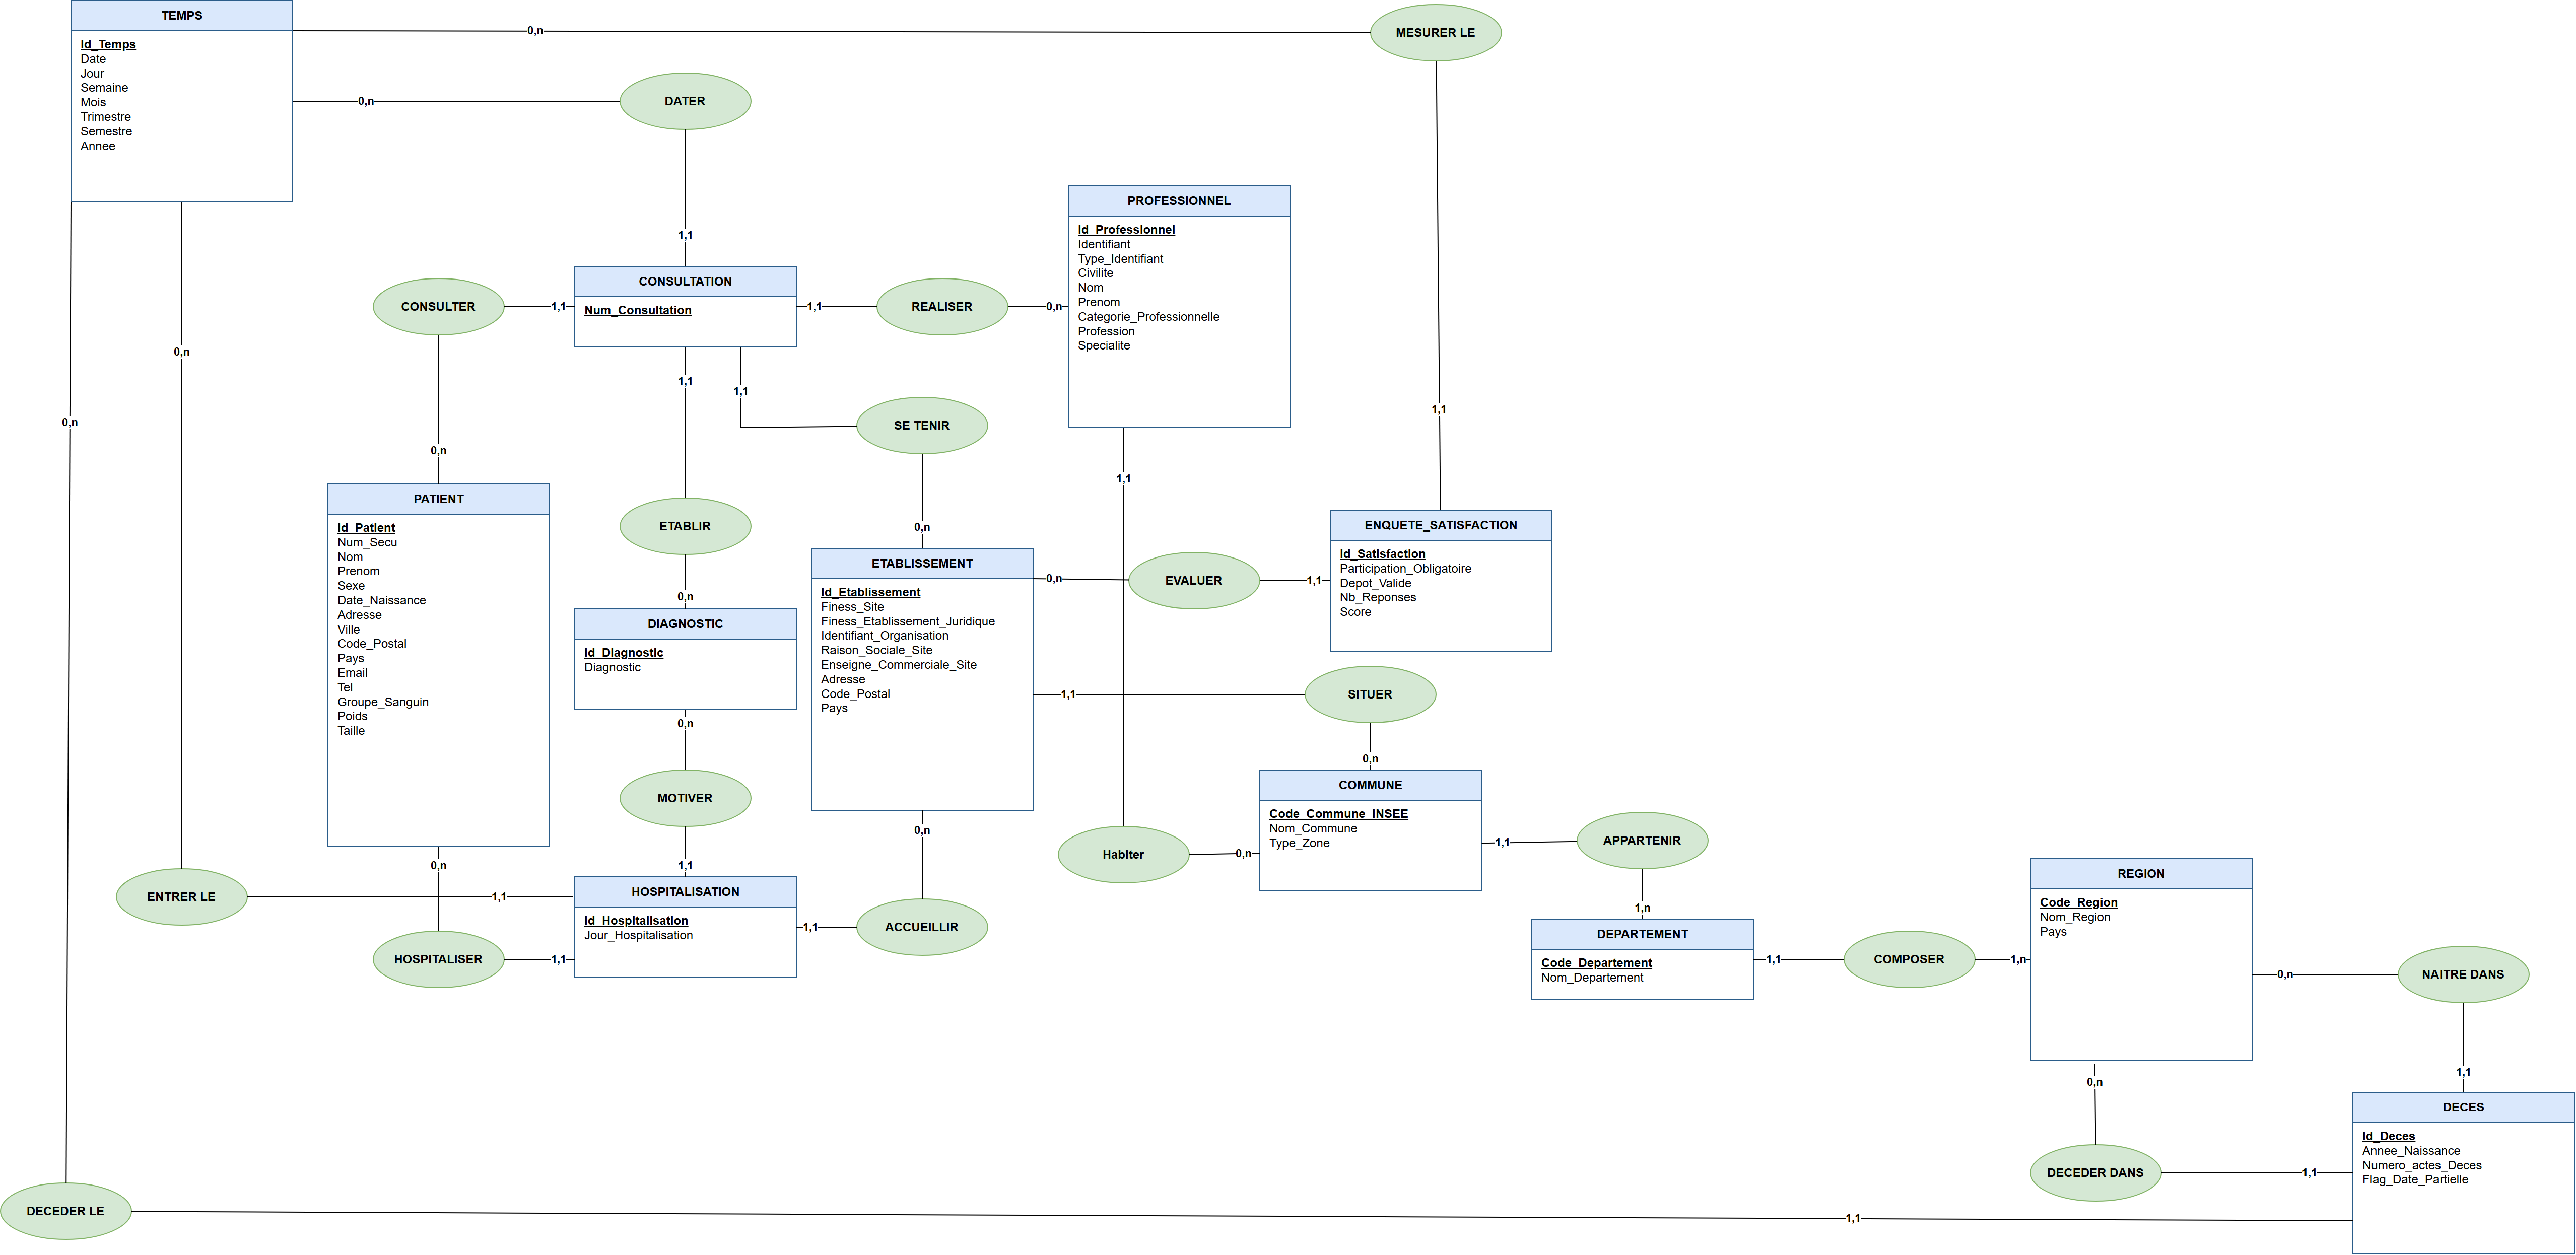
\includegraphics[width=\textwidth]{contents/img/modele_conceptuel.png}
\legende{Figure~1 -- Modèle dimensionnel conceptuel du CHU}
\end{center}

\subsubsection*{Tables de faits et dimensions}

\begin{tableau}{|>{\raggedright\arraybackslash}p{\dimexpr0.2697\linewidth-2\tabcolsep-1.2\arrayrulewidth\relax}|>{\raggedright\arraybackslash}p{\dimexpr0.3527\linewidth-2\tabcolsep-1.2\arrayrulewidth\relax}|>{\raggedright\arraybackslash}p{\dimexpr0.3775\linewidth-2\tabcolsep-1.2\arrayrulewidth\relax}|}
\rowcolor{tabentete}\textbf{Élément} & \textbf{Type} & \textbf{Table du modèle logique} \\ \hline
Consultations & Table de faits (processus métier) & FAIT\_\allowbreak CONSULTATION \\ \hline
Hospitalisations & Table de faits (processus métier) & FAIT\_\allowbreak HOSPITALISATION \\ \hline
Satisfaction & Table de faits (processus métier) & FAIT\_\allowbreak SATISFACTION \\ \hline
Décès & Table de faits (processus métier) & FAIT\_\allowbreak DECES \\ \hline
Temps & Dimension conforme (Jour $\rightarrow$ Mois $\rightarrow$ Trimestre $\rightarrow$ Année) & DIM\_\allowbreak Temps \\ \hline
Établissement & Dimension conforme & DIM\_\allowbreak Etablissement \\ \hline
Patient anonymisé & Dimension & DIM\_\allowbreak Patient \\ \hline
Diagnostic & Dimension & DIM\_\allowbreak Diagnostic \\ \hline
Professionnel & Dimension & DIM\_\allowbreak Professionnel \\ \hline
Région INSEE & Dimension (Commune $\rightarrow$ Département $\rightarrow$ Région) & DIM\_\allowbreak Region\_\allowbreak INSEE \\ \hline
\end{tableau}

\subsubsection*{Relations entre faits et dimensions}

\noindent Chaque relation relie une table de faits à une dimension et se lit dans les deux sens~: \og une consultation est réalisée par exactement un professionnel (1,1)~; un professionnel réalise zéro, une ou plusieurs consultations (0,n)\fg{}. Toutes les relations sont de ce type, ce qui permet de les traduire en clés étrangères de la table de faits. La dimension Région INSEE joue deux rôles pour les décès (lieu de décès et lieu de naissance).

\begin{tableau}{|>{\raggedright\arraybackslash}p{\dimexpr0.2075\linewidth-2\tabcolsep-1.2\arrayrulewidth\relax}|>{\raggedright\arraybackslash}p{\dimexpr0.2594\linewidth-2\tabcolsep-1.2\arrayrulewidth\relax}|>{\raggedright\arraybackslash}p{\dimexpr0.1037\linewidth-2\tabcolsep-1.2\arrayrulewidth\relax}|>{\raggedright\arraybackslash}p{\dimexpr0.2697\linewidth-2\tabcolsep-1.2\arrayrulewidth\relax}|>{\raggedright\arraybackslash}p{\dimexpr0.1597\linewidth-2\tabcolsep-1.2\arrayrulewidth\relax}|}
\rowcolor{tabentete}\textbf{Rôle} & \textbf{Table de faits} & \textbf{Card.} & \textbf{Dimension} & \textbf{Card.} \\ \hline
Auteur & Consultations & 1,1 & Professionnel & 0,n \\ \hline
Patient & Consultations & 1,1 & Patient anonymisé & 0,n \\ \hline
Diagnostic posé & Consultations & 1,1 & Diagnostic & 0,n \\ \hline
Lieu & Consultations & 1,1 & Établissement & 0,n \\ \hline
Date & Consultations & 1,1 & Temps & 0,n \\ \hline
Patient & Hospitalisations & 1,1 & Patient anonymisé & 0,n \\ \hline
Motif & Hospitalisations & 1,1 & Diagnostic & 0,n \\ \hline
Lieu d'accueil & Hospitalisations & 1,1 & Établissement & 0,n \\ \hline
Date d'entrée & Hospitalisations & 1,1 & Temps & 0,n \\ \hline
Établissement évalué & Satisfaction & 1,1 & Établissement & 0,n \\ \hline
Période de l'enquête & Satisfaction & 1,1 & Temps & 0,n \\ \hline
Lieu de décès & Décès & 1,1 & Région INSEE & 0,n \\ \hline
Lieu de naissance & Décès & 1,1 & Région INSEE & 0,n \\ \hline
Date de décès & Décès & 1,1 & Temps & 0,n \\ \hline
\end{tableau}

\noindent Les hiérarchies sont portées à l'intérieur des dimensions~: Commune $\rightarrow$ Département $\rightarrow$ Région dans la dimension Région INSEE, Jour $\rightarrow$ Mois $\rightarrow$ Trimestre $\rightarrow$ Année dans la dimension Temps. L'établissement et le professionnel sont situés par leur commune, qui reste un attribut de leur dimension. Au passage au modèle logique, ces hiérarchies sont dénormalisées dans leur dimension, ce qui évite un schéma en flocon~: les requêtes par région ne nécessitent qu'une seule jointure, au prix d'une légère redondance des libellés de département et de région.

\subsection{Schéma en constellation (modèle logique)}\label{sec:logique}

\noindent Le schéma en étoile constitue le \textbf{modèle logique} de l'entrepôt~: il traduit le modèle conceptuel (partie~\ref{sec:conceptuel}) en tables relationnelles, avec leurs attributs et leurs clés, sans dépendre du moteur de stockage. Il compte \textbf{quatre tables de faits} et \textbf{six dimensions}~; chaque table de faits forme une étoile avec ses dimensions, et les étoiles se rejoignent sur DIM\_Temps et DIM\_Etablissement.

\subsubsection*{Granularité des faits}

\noindent La granularité (le \og grain\fg{}) définit ce que représente une ligne de la table de faits. Elle est fixée au niveau le plus fin disponible dans les sources, afin de pouvoir agréger ensuite sans perte d'information.

\begin{tableau}{|>{\raggedright\arraybackslash}p{\dimexpr0.2385\linewidth-2\tabcolsep-1.2\arrayrulewidth\relax}|>{\raggedright\arraybackslash}p{\dimexpr0.4189\linewidth-2\tabcolsep-1.2\arrayrulewidth\relax}|>{\raggedright\arraybackslash}p{\dimexpr0.3426\linewidth-2\tabcolsep-1.2\arrayrulewidth\relax}|}
\rowcolor{tabentete}\textbf{Table de faits} & \textbf{Grain (1 ligne =)} & \textbf{Mesures} \\ \hline
FAIT\_\allowbreak CONSULTATION & 1 consultation d'un patient par un professionnel, dans un établissement, à une date & Nombre\_\allowbreak de\_\allowbreak consultation \\ \hline
FAIT\_\allowbreak HOSPITALISATION & 1 séjour hospitalier d'un patient dans un établissement & Jour\_\allowbreak Hospitalisation (durée) \\ \hline
FAIT\_\allowbreak SATISFACTION & 1 résultat d'enquête pour un établissement et une période & Nb\_\allowbreak Reponses, Score \\ \hline
FAIT\_\allowbreak DECES & 1 décès du fichier INSEE & Age\_\allowbreak Deces (et comptage des lignes) \\ \hline
\end{tableau}

\subsubsection*{Matrice faits $\times$ dimensions}

\noindent La matrice ci-dessous (dite \og matrice en bus\fg{} chez Kimball) indique quelles dimensions chaque fait utilise. Une dimension présente dans plusieurs colonnes est une dimension conforme~: elle a la même structure et les mêmes clés pour tous les faits, ce qui permet de croiser les indicateurs.

\begin{tableau}{|>{\raggedright\arraybackslash}p{\dimexpr0.2385\linewidth-2\tabcolsep-1.2\arrayrulewidth\relax}|>{\raggedright\arraybackslash}p{\dimexpr0.1908\linewidth-2\tabcolsep-1.2\arrayrulewidth\relax}|>{\raggedright\arraybackslash}p{\dimexpr0.1900\linewidth-2\tabcolsep-1.2\arrayrulewidth\relax}|>{\raggedright\arraybackslash}p{\dimexpr0.1901\linewidth-2\tabcolsep-1.2\arrayrulewidth\relax}|>{\raggedright\arraybackslash}p{\dimexpr0.1905\linewidth-2\tabcolsep-1.2\arrayrulewidth\relax}|}
\rowcolor{tabentete}\textbf{Dimension} & \textbf{Consultation} & \textbf{Hospitalisation} & \textbf{Satisfaction} & \textbf{Décès} \\ \hline
DIM\_\allowbreak Temps & X & X (date d'entrée) & X & X (date de décès) \\ \hline
DIM\_\allowbreak Etablissement & X & X & X &  \\ \hline
DIM\_\allowbreak Patient & X & X &  &  \\ \hline
DIM\_\allowbreak Diagnostic & X & X &  &  \\ \hline
DIM\_\allowbreak Professionnel & X &  &  &  \\ \hline
DIM\_\allowbreak Region\_\allowbreak INSEE &  &  &  & X (décès + naissance) \\ \hline
\end{tableau}

\noindent La figure 2 réunit ces éléments en une vue d'ensemble de la constellation~: les quatre faits, les six dimensions et leurs clés. Une version agrandie, en format paysage, est donnée en Annexe B.

\begin{center}
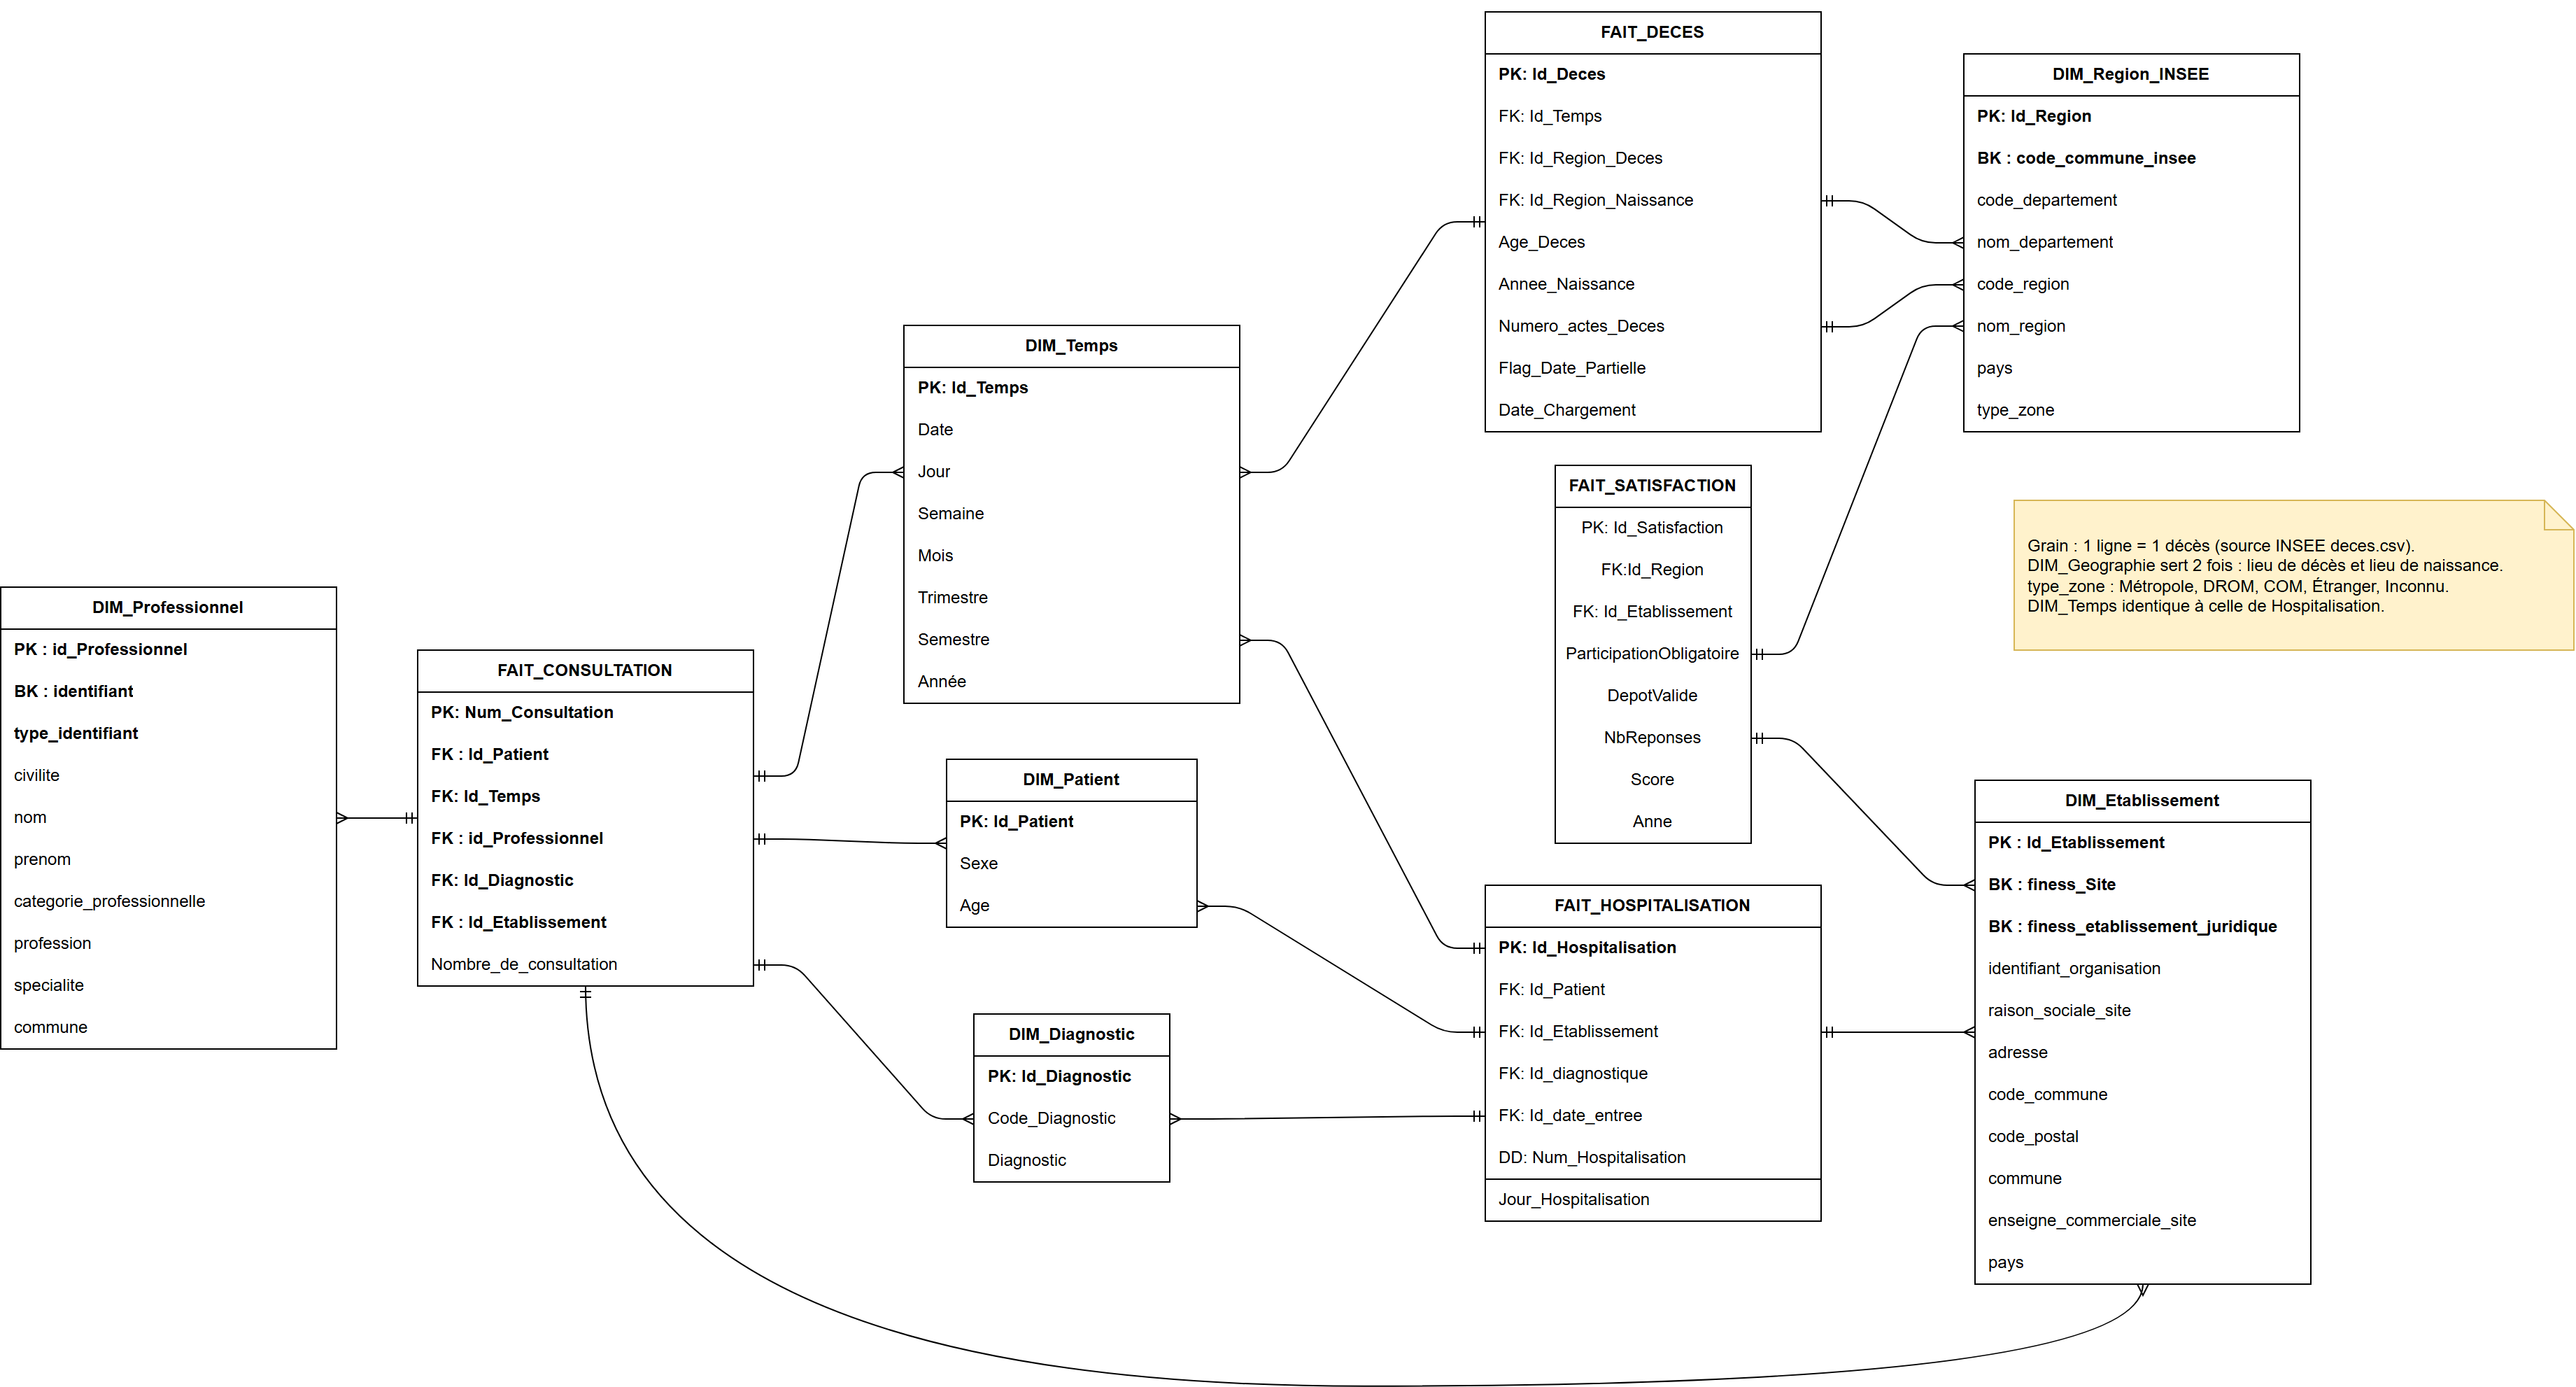
\includegraphics[width=\textwidth]{contents/img/schema_constellation.png}
\legende{Figure~2 -- Schéma logique en constellation du CHU}
\end{center}

\subsubsection*{Couverture des besoins}

\noindent Chaque besoin exprimé par le CHU se calcule à partir d'une seule table de faits et de ses dimensions, sans jointure entre faits.

\begin{tableau}{|>{\raggedright\arraybackslash}p{\dimexpr0.0622\linewidth-2\tabcolsep-1.2\arrayrulewidth\relax}|>{\raggedright\arraybackslash}p{\dimexpr0.3735\linewidth-2\tabcolsep-1.2\arrayrulewidth\relax}|>{\raggedright\arraybackslash}p{\dimexpr0.2490\linewidth-2\tabcolsep-1.2\arrayrulewidth\relax}|>{\raggedright\arraybackslash}p{\dimexpr0.3154\linewidth-2\tabcolsep-1.2\arrayrulewidth\relax}|}
\rowcolor{tabentete}\textbf{N°} & \textbf{Besoin} & \textbf{Fait} & \textbf{Dimensions utilisées} \\ \hline
1 & Taux de consultation par établissement et par période & FAIT\_\allowbreak CONSULTATION & DIM\_\allowbreak Etablissement, DIM\_\allowbreak Temps \\ \hline
2 & Taux de consultation par diagnostic et par période & FAIT\_\allowbreak CONSULTATION & DIM\_\allowbreak Diagnostic, DIM\_\allowbreak Temps \\ \hline
3 & Taux global d'hospitalisation par période & FAIT\_\allowbreak HOSPITALISATION & DIM\_\allowbreak Temps \\ \hline
4 & Taux d'hospitalisation par diagnostic et par période & FAIT\_\allowbreak HOSPITALISATION & DIM\_\allowbreak Diagnostic, DIM\_\allowbreak Temps \\ \hline
5 & Taux d'hospitalisation par sexe et par âge & FAIT\_\allowbreak HOSPITALISATION & DIM\_\allowbreak Patient \\ \hline
6 & Taux de consultation par professionnel & FAIT\_\allowbreak CONSULTATION & DIM\_\allowbreak Professionnel \\ \hline
7 & Nombre de décès par région en 2019 (optionnel) & FAIT\_\allowbreak DECES & DIM\_\allowbreak Region\_\allowbreak INSEE (rôle décès), DIM\_\allowbreak Temps \\ \hline
8 & Taux global de satisfaction par région en 2020 (optionnel) & FAIT\_\allowbreak SATISFACTION & DIM\_\allowbreak Etablissement ($\rightarrow$ région), DIM\_\allowbreak Temps \\ \hline
\end{tableau}

\subsubsection*{Règles de passage}

\noindent Trois règles ont permis de passer du modèle conceptuel (partie~\ref{sec:conceptuel}) aux tables~:

\begin{enumerate}
	\item chaque processus métier devient une table de faits~; ses relations vers les dimensions deviennent des \textbf{clés étrangères}~;
	\item chaque dimension devient une table identifiée par une \textbf{clé de substitution} (entier sans signification métier), la clé de la source étant conservée comme \textbf{clé métier} (BK)~;
	\item les hiérarchies (commune, département, région~; jour, mois, trimestre, année) sont \textbf{aplaties} dans leur dimension.
\end{enumerate}

\vspace{0.2cm}

\noindent Notation~: \textbf{PK} désigne une clé primaire, \textbf{FK} une clé étrangère, \textbf{BK} une clé métier et \textbf{DD} une dimension dégénérée (identifiant de la source conservé dans le fait sans table de dimension).

\subsubsection*{Schéma relationnel}

\noindent Le schéma relationnel reprend la figure 2 sous forme textuelle. La clé primaire est soulignée et les clés étrangères sont précédées d'un \#.

{\small\raggedright
\noindent \textbf{FAIT\_\allowbreak CONSULTATION} (\underline{Num\_\allowbreak Consultation}, \#Id\_\allowbreak Patient, \#Id\_\allowbreak Temps, \#Id\_\allowbreak Professionnel, \#Id\_\allowbreak Diagnostic, \#Id\_\allowbreak Etablissement, Nombre\_\allowbreak de\_\allowbreak consultation)

\noindent \textbf{FAIT\_\allowbreak HOSPITALISATION} (\underline{Id\_\allowbreak Hospitalisation}, \#Id\_\allowbreak Patient, \#Id\_\allowbreak Etablissement, \#Id\_\allowbreak Diagnostic, \#Id\_\allowbreak Date\_\allowbreak Entree, Num\_\allowbreak Hospitalisation, Jour\_\allowbreak Hospitalisation)

\noindent \textbf{FAIT\_\allowbreak SATISFACTION} (\underline{Id\_\allowbreak Satisfaction}, \#Id\_\allowbreak Temps, \#Id\_\allowbreak Etablissement, Participation\_\allowbreak Obligatoire, Depot\_\allowbreak Valide, Nb\_\allowbreak Reponses, Score)

\noindent \textbf{FAIT\_\allowbreak DECES} (\underline{Id\_\allowbreak Deces}, \#Id\_\allowbreak Temps, \#Id\_\allowbreak Region\_\allowbreak Deces, \#Id\_\allowbreak Region\_\allowbreak Naissance, Age\_\allowbreak Deces, Annee\_\allowbreak Naissance, Numero\_\allowbreak Acte\_\allowbreak Deces, Flag\_\allowbreak Date\_\allowbreak Partielle, Date\_\allowbreak Chargement)

\noindent \textbf{DIM\_\allowbreak Temps} (\underline{Id\_\allowbreak Temps}, Date, Jour, Semaine, Mois, Trimestre, Semestre, Annee)

\noindent \textbf{DIM\_\allowbreak Patient} (\underline{Id\_\allowbreak Patient}, Nom, Prenom, Sexe, Adresse, Ville, Code\_\allowbreak Postal, Pays, Email, Tel, Date\_\allowbreak Naissance, Age, Num\_\allowbreak Secu, Groupe\_\allowbreak Sanguin, Poids, Taille)

\noindent \textbf{DIM\_\allowbreak Diagnostic} (\underline{Id\_\allowbreak Diagnostic}, Code\_\allowbreak Diagnostic, Diagnostic)

\noindent \textbf{DIM\_\allowbreak Etablissement} (\underline{Id\_\allowbreak Etablissement}, Finess\_\allowbreak Site, Finess\_\allowbreak Etablissement\_\allowbreak Juridique, Identifiant\_\allowbreak Organisation, Raison\_\allowbreak Sociale\_\allowbreak Site, Enseigne\_\allowbreak Commerciale\_\allowbreak Site, Adresse, Code\_\allowbreak Commune, Code\_\allowbreak Postal, Commune, Pays)

\noindent \textbf{DIM\_\allowbreak Professionnel} (\underline{Id\_\allowbreak Professionnel}, Identifiant, Type\_\allowbreak Identifiant, Civilite, Nom, Prenom, Categorie\_\allowbreak Professionnelle, Profession, Specialite, Commune)

\noindent \textbf{DIM\_\allowbreak Region\_\allowbreak INSEE} (\underline{Id\_\allowbreak Region}, Code\_\allowbreak Commune\_\allowbreak INSEE, Code\_\allowbreak Departement, Nom\_\allowbreak Departement, Code\_\allowbreak Region, Nom\_\allowbreak Region, Pays, Type\_\allowbreak Zone)
\par}

\subsubsection*{Clés étrangères et cardinalités}

\noindent Toutes les relations du schéma sont de type \textbf{un-à-plusieurs}~: une ligne de dimension est référencée par zéro, une ou plusieurs lignes de faits, et chaque ligne de faits référence exactement une ligne de dimension. Les clés étrangères des faits sont donc \textbf{non nulles}~; une valeur absente dans la source est rattachée à un membre \og Inconnu\fg{} (clé~$-1$) de la dimension plutôt que laissée à NULL, pour ne perdre aucune ligne dans les agrégats.

\begin{tableau}{|>{\raggedright\arraybackslash}p{\dimexpr0.2594\linewidth-2\tabcolsep-1.2\arrayrulewidth\relax}|>{\raggedright\arraybackslash}p{\dimexpr0.2178\linewidth-2\tabcolsep-1.2\arrayrulewidth\relax}|>{\raggedright\arraybackslash}p{\dimexpr0.2425\linewidth-2\tabcolsep-1.2\arrayrulewidth\relax}|>{\raggedright\arraybackslash}p{\dimexpr0.1348\linewidth-2\tabcolsep-1.2\arrayrulewidth\relax}|>{\raggedright\arraybackslash}p{\dimexpr0.1455\linewidth-2\tabcolsep-1.2\arrayrulewidth\relax}|}
\rowcolor{tabentete}\textbf{Table de faits} & \textbf{Clé étrangère} & \textbf{Dimension référencée} & \textbf{Côté dimension} & \textbf{Côté fait} \\ \hline
FAIT\_\allowbreak CONSULTATION & Id\_\allowbreak Patient & DIM\_\allowbreak Patient & 1 & 0..n \\ \hline
FAIT\_\allowbreak CONSULTATION & Id\_\allowbreak Temps & DIM\_\allowbreak Temps & 1 & 0..n \\ \hline
FAIT\_\allowbreak CONSULTATION & Id\_\allowbreak Professionnel & DIM\_\allowbreak Professionnel & 1 & 0..n \\ \hline
FAIT\_\allowbreak CONSULTATION & Id\_\allowbreak Diagnostic & DIM\_\allowbreak Diagnostic & 1 & 0..n \\ \hline
FAIT\_\allowbreak CONSULTATION & Id\_\allowbreak Etablissement & DIM\_\allowbreak Etablissement & 1 & 0..n \\ \hline
FAIT\_\allowbreak HOSPITALISATION & Id\_\allowbreak Patient & DIM\_\allowbreak Patient & 1 & 0..n \\ \hline
FAIT\_\allowbreak HOSPITALISATION & Id\_\allowbreak Etablissement & DIM\_\allowbreak Etablissement & 1 & 0..n \\ \hline
FAIT\_\allowbreak HOSPITALISATION & Id\_\allowbreak Diagnostic & DIM\_\allowbreak Diagnostic & 1 & 0..n \\ \hline
FAIT\_\allowbreak HOSPITALISATION & Id\_\allowbreak Date\_\allowbreak Entree & DIM\_\allowbreak Temps & 1 & 0..n \\ \hline
FAIT\_\allowbreak SATISFACTION & Id\_\allowbreak Temps & DIM\_\allowbreak Temps & 1 & 0..n \\ \hline
FAIT\_\allowbreak SATISFACTION & Id\_\allowbreak Etablissement & DIM\_\allowbreak Etablissement & 1 & 0..n \\ \hline
FAIT\_\allowbreak DECES & Id\_\allowbreak Temps & DIM\_\allowbreak Temps & 1 & 0..n \\ \hline
FAIT\_\allowbreak DECES & Id\_\allowbreak Region\_\allowbreak Deces & DIM\_\allowbreak Region\_\allowbreak INSEE & 1 & 0..n \\ \hline
FAIT\_\allowbreak DECES & Id\_\allowbreak Region\_\allowbreak Naissance & DIM\_\allowbreak Region\_\allowbreak INSEE & 1 & 0..n \\ \hline
\end{tableau}

\subsubsection*{Choix de modélisation}

\begin{itemize}
	\item \textbf{Clés de substitution}~: les dimensions sont identifiées par un entier généré par l'ETL. Elles isolent l'entrepôt des changements de codification des sources et accélèrent les jointures.
	\item \textbf{Dimensions conformes}~: DIM\_Temps et DIM\_Etablissement sont uniques et partagées, ce qui garantit que \og mars 2019\fg{} ou \og tel établissement\fg{} ont le même sens pour tous les indicateurs.
	\item \textbf{Dimension à rôles multiples}~: DIM\_Region\_INSEE est jouée deux fois par FAIT\_DECES (lieu de décès et lieu de naissance), via deux clés étrangères distinctes.
	\item \textbf{Dimensions dégénérées}~: Num\_Hospitalisation et Numero\_Acte\_Deces restent dans les faits pour le dédoublonnage et la traçabilité vers la source.
	\item \textbf{Mesures}~: les mesures additives (Nombre\_de\_consultation, Jour\_Hospitalisation, Nb\_Reponses) se somment sur tous les axes~; Score est non additif et s'agrège en moyenne pondérée par Nb\_Reponses.
\end{itemize}

\subsection{Dictionnaire de données}\label{sec:dictionnaire}

\noindent Le dictionnaire décrit chaque table et chaque attribut du modèle. Les types sont exprimés en SQL standard (compatibles PostgreSQL)~; ils seront ajustés au moteur retenu lors de l'implémentation physique (livrable 2).

\vspace{0.2cm}

\noindent Légende de la colonne \og Clé\fg{}~: \textbf{PK} clé primaire, \textbf{FK} clé étrangère, \textbf{BK} clé métier (identifiant de la source, unique dans la dimension), \textbf{DD} dimension dégénérée.

\needspace{18\baselineskip}
\subsubsection*{FAIT\_CONSULTATION}

\noindent \textbf{Type}~: Table de faits. \textbf{Grain}~: 1 ligne = 1 consultation réalisée par un professionnel pour un patient, dans un établissement, à une date.\\
\textbf{Source}~: base opérationnelle PostgreSQL (consultations, diagnostics, patients, professionnels).\\
\textbf{Besoins couverts}~: 1, 2 et 6.

\begin{tableau}{|>{\raggedright\arraybackslash}p{\dimexpr0.2594\linewidth-2\tabcolsep-1.2\arrayrulewidth\relax}|>{\raggedright\arraybackslash}p{\dimexpr0.1653\linewidth-2\tabcolsep-1.2\arrayrulewidth\relax}|>{\raggedright\arraybackslash}p{\dimexpr0.0674\linewidth-2\tabcolsep-1.2\arrayrulewidth\relax}|>{\raggedright\arraybackslash}p{\dimexpr0.0674\linewidth-2\tabcolsep-1.2\arrayrulewidth\relax}|>{\raggedright\arraybackslash}p{\dimexpr0.4407\linewidth-2\tabcolsep-1.2\arrayrulewidth\relax}|}
\rowcolor{tabentete}\textbf{Attribut} & \textbf{Type} & \textbf{Clé} & \textbf{Null} & \textbf{Description} \\ \hline
Num\_\allowbreak Consultation & BIGINT & PK & Non & Identifiant de la consultation (numéro issu de la source). \\ \hline
Id\_\allowbreak Patient & INTEGER & FK & Non & Patient consulté $\rightarrow$ DIM\_\allowbreak Patient. \\ \hline
Id\_\allowbreak Temps & INTEGER & FK & Non & Date de la consultation $\rightarrow$ DIM\_\allowbreak Temps. \\ \hline
Id\_\allowbreak Professionnel & INTEGER & FK & Non & Professionnel qui réalise la consultation $\rightarrow$ DIM\_\allowbreak Professionnel. \\ \hline
Id\_\allowbreak Diagnostic & INTEGER & FK & Non & Diagnostic posé $\rightarrow$ DIM\_\allowbreak Diagnostic (membre \og Non renseigné\fg{} si absent). \\ \hline
Id\_\allowbreak Etablissement & INTEGER & FK & Non & Établissement où se tient la consultation $\rightarrow$ DIM\_\allowbreak Etablissement. \\ \hline
Nombre\_\allowbreak de\_\allowbreak consultation & SMALLINT &  & Non & Mesure additive, vaut 1 par ligne. Sa somme donne le nombre de consultations. \\ \hline
\end{tableau}

\needspace{18\baselineskip}
\subsubsection*{FAIT\_HOSPITALISATION}

\noindent \textbf{Type}~: Table de faits. \textbf{Grain}~: 1 ligne = 1 séjour hospitalier d'un patient dans un établissement.\\
\textbf{Source}~: base opérationnelle PostgreSQL (séjours, admissions, diagnostics).\\
\textbf{Besoins couverts}~: 3, 4 et 5.

\begin{tableau}{|>{\raggedright\arraybackslash}p{\dimexpr0.2594\linewidth-2\tabcolsep-1.2\arrayrulewidth\relax}|>{\raggedright\arraybackslash}p{\dimexpr0.1653\linewidth-2\tabcolsep-1.2\arrayrulewidth\relax}|>{\raggedright\arraybackslash}p{\dimexpr0.0674\linewidth-2\tabcolsep-1.2\arrayrulewidth\relax}|>{\raggedright\arraybackslash}p{\dimexpr0.0674\linewidth-2\tabcolsep-1.2\arrayrulewidth\relax}|>{\raggedright\arraybackslash}p{\dimexpr0.4407\linewidth-2\tabcolsep-1.2\arrayrulewidth\relax}|}
\rowcolor{tabentete}\textbf{Attribut} & \textbf{Type} & \textbf{Clé} & \textbf{Null} & \textbf{Description} \\ \hline
Id\_\allowbreak Hospitalisation & BIGINT & PK & Non & Clé de substitution du séjour. \\ \hline
Id\_\allowbreak Patient & INTEGER & FK & Non & Patient hospitalisé $\rightarrow$ DIM\_\allowbreak Patient. \\ \hline
Id\_\allowbreak Etablissement & INTEGER & FK & Non & Établissement d'accueil $\rightarrow$ DIM\_\allowbreak Etablissement. \\ \hline
Id\_\allowbreak Diagnostic & INTEGER & FK & Non & Diagnostic à l'origine du séjour $\rightarrow$ DIM\_\allowbreak Diagnostic. \\ \hline
Id\_\allowbreak Date\_\allowbreak Entree & INTEGER & FK & Non & Date d'entrée du séjour $\rightarrow$ DIM\_\allowbreak Temps (rôle \og date d'entrée\fg{}). \\ \hline
Num\_\allowbreak Hospitalisation & VARCHAR(20) & DD & Non & Dimension dégénérée~: numéro du séjour dans la source, conservé pour la traçabilité. \\ \hline
Jour\_\allowbreak Hospitalisation & SMALLINT &  & Oui & Mesure additive~: durée du séjour en jours. \\ \hline
\end{tableau}

\needspace{17\baselineskip}
\subsubsection*{FAIT\_SATISFACTION}

\noindent \textbf{Type}~: Table de faits. \textbf{Grain}~: 1 ligne = 1 résultat d'enquête de satisfaction pour un établissement et une période de mesure.\\
\textbf{Source}~: fichiers plats déposés sur le serveur FTP (enquêtes de satisfaction).\\
\textbf{Besoins couverts}~: 8.

\begin{tableau}{|>{\raggedright\arraybackslash}p{\dimexpr0.2594\linewidth-2\tabcolsep-1.2\arrayrulewidth\relax}|>{\raggedright\arraybackslash}p{\dimexpr0.1653\linewidth-2\tabcolsep-1.2\arrayrulewidth\relax}|>{\raggedright\arraybackslash}p{\dimexpr0.0674\linewidth-2\tabcolsep-1.2\arrayrulewidth\relax}|>{\raggedright\arraybackslash}p{\dimexpr0.0674\linewidth-2\tabcolsep-1.2\arrayrulewidth\relax}|>{\raggedright\arraybackslash}p{\dimexpr0.4407\linewidth-2\tabcolsep-1.2\arrayrulewidth\relax}|}
\rowcolor{tabentete}\textbf{Attribut} & \textbf{Type} & \textbf{Clé} & \textbf{Null} & \textbf{Description} \\ \hline
Id\_\allowbreak Satisfaction & BIGINT & PK & Non & Clé de substitution du résultat d'enquête. \\ \hline
Id\_\allowbreak Temps & INTEGER & FK & Non & Période de mesure $\rightarrow$ DIM\_\allowbreak Temps. \\ \hline
Id\_\allowbreak Etablissement & INTEGER & FK & Non & Établissement évalué $\rightarrow$ DIM\_\allowbreak Etablissement. \\ \hline
Participation\_\allowbreak Obligatoire & BOOLEAN &  & Oui & Indique si l'établissement était tenu de participer à l'enquête. \\ \hline
Depot\_\allowbreak Valide & BOOLEAN &  & Oui & Indique si le dépôt des résultats a été validé. \\ \hline
Nb\_\allowbreak Reponses & INTEGER &  & Oui & Mesure additive~: nombre de questionnaires exploitables. \\ \hline
Score & NUMERIC(5,2) &  & Oui & Mesure non additive~: score global de satisfaction. Agrégé en moyenne pondérée par Nb\_\allowbreak Reponses. \\ \hline
\end{tableau}

\needspace{19\baselineskip}
\subsubsection*{FAIT\_DECES}

\noindent \textbf{Type}~: Table de faits. \textbf{Grain}~: 1 ligne = 1 décès enregistré dans le fichier INSEE (deces.csv, environ 25 millions de lignes).\\
\textbf{Source}~: fichier des personnes décédées de l'INSEE (open data), déposé sur le serveur FTP.\\
\textbf{Besoins couverts}~: 7.

\begin{tableau}{|>{\raggedright\arraybackslash}p{\dimexpr0.2594\linewidth-2\tabcolsep-1.2\arrayrulewidth\relax}|>{\raggedright\arraybackslash}p{\dimexpr0.1653\linewidth-2\tabcolsep-1.2\arrayrulewidth\relax}|>{\raggedright\arraybackslash}p{\dimexpr0.0674\linewidth-2\tabcolsep-1.2\arrayrulewidth\relax}|>{\raggedright\arraybackslash}p{\dimexpr0.0674\linewidth-2\tabcolsep-1.2\arrayrulewidth\relax}|>{\raggedright\arraybackslash}p{\dimexpr0.4407\linewidth-2\tabcolsep-1.2\arrayrulewidth\relax}|}
\rowcolor{tabentete}\textbf{Attribut} & \textbf{Type} & \textbf{Clé} & \textbf{Null} & \textbf{Description} \\ \hline
Id\_\allowbreak Deces & BIGINT & PK & Non & Clé de substitution du décès. \\ \hline
Id\_\allowbreak Temps & INTEGER & FK & Non & Date du décès $\rightarrow$ DIM\_\allowbreak Temps (rôle \og date de décès\fg{}). \\ \hline
Id\_\allowbreak Region\_\allowbreak Deces & INTEGER & FK & Non & Lieu du décès $\rightarrow$ DIM\_\allowbreak Region\_\allowbreak INSEE (rôle \og lieu de décès\fg{}). Membre~$-1$ \og Inconnu\fg{} si le code est vide. \\ \hline
Id\_\allowbreak Region\_\allowbreak Naissance & INTEGER & FK & Non & Lieu de naissance $\rightarrow$ DIM\_\allowbreak Region\_\allowbreak INSEE (rôle \og lieu de naissance\fg{}). \\ \hline
Age\_\allowbreak Deces & SMALLINT &  & Oui & Âge au décès en années, calculé à partir des dates de naissance et de décès. \\ \hline
Annee\_\allowbreak Naissance & SMALLINT &  & Oui & Année de naissance. Seule l'année est conservée (minimisation RGPD). \\ \hline
Numero\_\allowbreak Acte\_\allowbreak Deces & VARCHAR(10) & DD & Oui & Dimension dégénérée~: numéro de l'acte de décès, utile au dédoublonnage. \\ \hline
Flag\_\allowbreak Date\_\allowbreak Partielle & BOOLEAN &  & Non & Vrai si la date de naissance ou de décès est incomplète dans la source (ex. \og 1930\fg{}, \og 1989-05\fg{}). \\ \hline
Date\_\allowbreak Chargement & TIMESTAMP &  & Non & Horodatage du chargement de la ligne (traçabilité ETL). \\ \hline
\end{tableau}

\needspace{17\baselineskip}
\subsubsection*{DIM\_Temps}

\noindent \textbf{Type}~: Dimension conforme. \textbf{Grain}~: 1 ligne = 1 jour calendaire.\\
\textbf{Source}~: générée par l'ETL (calendrier), partagée par les quatre tables de faits.\\
\textbf{Besoins couverts}~: tous (axe \og période\fg{}).

\begin{tableau}{|>{\raggedright\arraybackslash}p{\dimexpr0.2594\linewidth-2\tabcolsep-1.2\arrayrulewidth\relax}|>{\raggedright\arraybackslash}p{\dimexpr0.1653\linewidth-2\tabcolsep-1.2\arrayrulewidth\relax}|>{\raggedright\arraybackslash}p{\dimexpr0.0674\linewidth-2\tabcolsep-1.2\arrayrulewidth\relax}|>{\raggedright\arraybackslash}p{\dimexpr0.0674\linewidth-2\tabcolsep-1.2\arrayrulewidth\relax}|>{\raggedright\arraybackslash}p{\dimexpr0.4407\linewidth-2\tabcolsep-1.2\arrayrulewidth\relax}|}
\rowcolor{tabentete}\textbf{Attribut} & \textbf{Type} & \textbf{Clé} & \textbf{Null} & \textbf{Description} \\ \hline
Id\_\allowbreak Temps & INTEGER & PK & Non & Clé au format AAAAMMJJ (ex. 20190315), lisible et triable. \\ \hline
Date & DATE &  & Non & Date complète. \\ \hline
Jour & SMALLINT &  & Non & Jour du mois (1 à 31). \\ \hline
Semaine & SMALLINT &  & Non & Numéro de semaine ISO (1 à 53). \\ \hline
Mois & SMALLINT &  & Non & Mois (1 à 12). \\ \hline
Trimestre & SMALLINT &  & Non & Trimestre (1 à 4). \\ \hline
Semestre & SMALLINT &  & Non & Semestre (1 ou 2). \\ \hline
Annee & SMALLINT &  & Non & Année civile. \\ \hline
\end{tableau}

\needspace{25\baselineskip}
\subsubsection*{DIM\_Patient}

\noindent \textbf{Type}~: Dimension. \textbf{Grain}~: 1 ligne = 1 patient.\\
\textbf{Source}~: base opérationnelle PostgreSQL (table des patients).\\
\textbf{Besoins couverts}~: 5 (sexe, âge).

\begin{tableau}{|>{\raggedright\arraybackslash}p{\dimexpr0.2594\linewidth-2\tabcolsep-1.2\arrayrulewidth\relax}|>{\raggedright\arraybackslash}p{\dimexpr0.1653\linewidth-2\tabcolsep-1.2\arrayrulewidth\relax}|>{\raggedright\arraybackslash}p{\dimexpr0.0674\linewidth-2\tabcolsep-1.2\arrayrulewidth\relax}|>{\raggedright\arraybackslash}p{\dimexpr0.0674\linewidth-2\tabcolsep-1.2\arrayrulewidth\relax}|>{\raggedright\arraybackslash}p{\dimexpr0.4407\linewidth-2\tabcolsep-1.2\arrayrulewidth\relax}|}
\rowcolor{tabentete}\textbf{Attribut} & \textbf{Type} & \textbf{Clé} & \textbf{Null} & \textbf{Description} \\ \hline
Id\_\allowbreak Patient & INTEGER & PK & Non & Clé de substitution du patient. \\ \hline
Nom & VARCHAR(100) &  & Oui & Nom du patient. Donnée identifiante. \\ \hline
Prenom & VARCHAR(100) &  & Oui & Prénom du patient. Donnée identifiante. \\ \hline
Sexe & CHAR(1) &  & Non & Sexe (M, F, I pour inconnu). \\ \hline
Adresse & VARCHAR(255) &  & Oui & Adresse postale. Donnée identifiante. \\ \hline
Ville & VARCHAR(100) &  & Oui & Ville de résidence. \\ \hline
Code\_\allowbreak Postal & CHAR(5) &  & Oui & Code postal de résidence. \\ \hline
Pays & VARCHAR(50) &  & Oui & Pays de résidence. \\ \hline
Email & VARCHAR(255) &  & Oui & Adresse électronique. Donnée identifiante. \\ \hline
Tel & VARCHAR(20) &  & Oui & Téléphone. Donnée identifiante. \\ \hline
Date\_\allowbreak Naissance & DATE &  & Oui & Date de naissance (attribut \og Date\fg{} du schéma). \\ \hline
Age & SMALLINT &  & Oui & Âge du patient en années. \\ \hline
Num\_\allowbreak Secu & CHAR(15) &  & Oui & Numéro de sécurité sociale (NIR). Donnée identifiante. \\ \hline
Groupe\_\allowbreak Sanguin & VARCHAR(3) &  & Oui & Groupe sanguin (A+, O-\ldots{}). \\ \hline
Poids & NUMERIC(5,1) &  & Oui & Poids en kg. \\ \hline
Taille & NUMERIC(4,1) &  & Oui & Taille en cm. \\ \hline
\end{tableau}

\needspace{8\baselineskip}
\subsubsection*{DIM\_Diagnostic}

\noindent \textbf{Type}~: Dimension. \textbf{Grain}~: 1 ligne = 1 code diagnostic.\\
\textbf{Source}~: base opérationnelle PostgreSQL (table des diagnostics).\\
\textbf{Besoins couverts}~: 2 et 4.

\begin{tableau}{|>{\raggedright\arraybackslash}p{\dimexpr0.2594\linewidth-2\tabcolsep-1.2\arrayrulewidth\relax}|>{\raggedright\arraybackslash}p{\dimexpr0.1653\linewidth-2\tabcolsep-1.2\arrayrulewidth\relax}|>{\raggedright\arraybackslash}p{\dimexpr0.0674\linewidth-2\tabcolsep-1.2\arrayrulewidth\relax}|>{\raggedright\arraybackslash}p{\dimexpr0.0674\linewidth-2\tabcolsep-1.2\arrayrulewidth\relax}|>{\raggedright\arraybackslash}p{\dimexpr0.4407\linewidth-2\tabcolsep-1.2\arrayrulewidth\relax}|}
\rowcolor{tabentete}\textbf{Attribut} & \textbf{Type} & \textbf{Clé} & \textbf{Null} & \textbf{Description} \\ \hline
Id\_\allowbreak Diagnostic & INTEGER & PK & Non & Clé de substitution du diagnostic. \\ \hline
Code\_\allowbreak Diagnostic & VARCHAR(10) & BK & Non & Code du diagnostic dans la source (clé métier). \\ \hline
Diagnostic & VARCHAR(255) &  & Non & Libellé du diagnostic. \\ \hline
\end{tableau}

\needspace{20\baselineskip}
\subsubsection*{DIM\_Etablissement}

\noindent \textbf{Type}~: Dimension conforme. \textbf{Grain}~: 1 ligne = 1 site géographique d'établissement (FINESS site).\\
\textbf{Source}~: fichier CSV de gestion administrative des établissements (référentiel FINESS).\\
\textbf{Besoins couverts}~: 1 et 8~; partagée par Consultation, Hospitalisation et Satisfaction.

\begin{tableau}{|>{\raggedright\arraybackslash}p{\dimexpr0.2594\linewidth-2\tabcolsep-1.2\arrayrulewidth\relax}|>{\raggedright\arraybackslash}p{\dimexpr0.1653\linewidth-2\tabcolsep-1.2\arrayrulewidth\relax}|>{\raggedright\arraybackslash}p{\dimexpr0.0674\linewidth-2\tabcolsep-1.2\arrayrulewidth\relax}|>{\raggedright\arraybackslash}p{\dimexpr0.0674\linewidth-2\tabcolsep-1.2\arrayrulewidth\relax}|>{\raggedright\arraybackslash}p{\dimexpr0.4407\linewidth-2\tabcolsep-1.2\arrayrulewidth\relax}|}
\rowcolor{tabentete}\textbf{Attribut} & \textbf{Type} & \textbf{Clé} & \textbf{Null} & \textbf{Description} \\ \hline
Id\_\allowbreak Etablissement & INTEGER & PK & Non & Clé de substitution de l'établissement. \\ \hline
Finess\_\allowbreak Site & CHAR(9) & BK & Non & Numéro FINESS du site géographique (clé métier). \\ \hline
Finess\_\allowbreak Etablissement\_\allowbreak Juridique & CHAR(9) & BK & Oui & Numéro FINESS de l'entité juridique de rattachement. \\ \hline
Identifiant\_\allowbreak Organisation & VARCHAR(30) &  & Oui & Identifiant de l'organisation dans le référentiel. \\ \hline
Raison\_\allowbreak Sociale\_\allowbreak Site & VARCHAR(255) &  & Non & Raison sociale du site. \\ \hline
Enseigne\_\allowbreak Commerciale\_\allowbreak Site & VARCHAR(255) &  & Oui & Enseigne commerciale du site. \\ \hline
Adresse & VARCHAR(255) &  & Oui & Adresse du site. \\ \hline
Code\_\allowbreak Commune & CHAR(5) &  & Oui & Code commune INSEE du site (permet le rattachement à la région). \\ \hline
Code\_\allowbreak Postal & CHAR(5) &  & Oui & Code postal du site. \\ \hline
Commune & VARCHAR(100) &  & Oui & Nom de la commune. \\ \hline
Pays & VARCHAR(50) &  & Oui & Pays. \\ \hline
\end{tableau}

\needspace{19\baselineskip}
\subsubsection*{DIM\_Professionnel}

\noindent \textbf{Type}~: Dimension. \textbf{Grain}~: 1 ligne = 1 professionnel de santé.\\
\textbf{Source}~: référentiel des professionnels de santé.\\
\textbf{Besoins couverts}~: 6.

\begin{tableau}{|>{\raggedright\arraybackslash}p{\dimexpr0.2594\linewidth-2\tabcolsep-1.2\arrayrulewidth\relax}|>{\raggedright\arraybackslash}p{\dimexpr0.1653\linewidth-2\tabcolsep-1.2\arrayrulewidth\relax}|>{\raggedright\arraybackslash}p{\dimexpr0.0674\linewidth-2\tabcolsep-1.2\arrayrulewidth\relax}|>{\raggedright\arraybackslash}p{\dimexpr0.0674\linewidth-2\tabcolsep-1.2\arrayrulewidth\relax}|>{\raggedright\arraybackslash}p{\dimexpr0.4407\linewidth-2\tabcolsep-1.2\arrayrulewidth\relax}|}
\rowcolor{tabentete}\textbf{Attribut} & \textbf{Type} & \textbf{Clé} & \textbf{Null} & \textbf{Description} \\ \hline
Id\_\allowbreak Professionnel & INTEGER & PK & Non & Clé de substitution du professionnel. \\ \hline
Identifiant & VARCHAR(20) & BK & Non & Identifiant national du professionnel (clé métier). \\ \hline
Type\_\allowbreak Identifiant & VARCHAR(10) &  & Non & Nature de l'identifiant (ex. RPPS, ADELI). \\ \hline
Civilite & VARCHAR(10) &  & Oui & Civilité. \\ \hline
Nom & VARCHAR(100) &  & Non & Nom d'exercice. \\ \hline
Prenom & VARCHAR(100) &  & Oui & Prénom d'exercice. \\ \hline
Categorie\_\allowbreak Professionnelle & VARCHAR(50) &  & Oui & Catégorie (civil, militaire, étudiant\ldots{}). \\ \hline
Profession & VARCHAR(100) &  & Oui & Profession exercée (médecin, infirmier\ldots{}). \\ \hline
Specialite & VARCHAR(150) &  & Oui & Spécialité ou savoir-faire. \\ \hline
Commune & VARCHAR(100) &  & Oui & Commune d'exercice. \\ \hline
\end{tableau}

\needspace{17\baselineskip}
\subsubsection*{DIM\_Region\_INSEE}

\noindent \textbf{Type}~: Dimension (à rôles multiples). \textbf{Grain}~: 1 ligne = 1 commune INSEE, avec son département et sa région. Membre~$-1$ \og Inconnu\fg{} pour les codes vides.\\
\textbf{Source}~: Code officiel géographique de l'INSEE, construit à partir des codes lieu du fichier des décès.\\
\textbf{Besoins couverts}~: 7~; jouée deux fois par FAIT\_DECES (lieu de décès, lieu de naissance).

\begin{tableau}{|>{\raggedright\arraybackslash}p{\dimexpr0.2594\linewidth-2\tabcolsep-1.2\arrayrulewidth\relax}|>{\raggedright\arraybackslash}p{\dimexpr0.1653\linewidth-2\tabcolsep-1.2\arrayrulewidth\relax}|>{\raggedright\arraybackslash}p{\dimexpr0.0674\linewidth-2\tabcolsep-1.2\arrayrulewidth\relax}|>{\raggedright\arraybackslash}p{\dimexpr0.0674\linewidth-2\tabcolsep-1.2\arrayrulewidth\relax}|>{\raggedright\arraybackslash}p{\dimexpr0.4407\linewidth-2\tabcolsep-1.2\arrayrulewidth\relax}|}
\rowcolor{tabentete}\textbf{Attribut} & \textbf{Type} & \textbf{Clé} & \textbf{Null} & \textbf{Description} \\ \hline
Id\_\allowbreak Region & INTEGER & PK & Non & Clé de substitution de la commune. \\ \hline
Code\_\allowbreak Commune\_\allowbreak INSEE & CHAR(5) & BK & Oui & Code commune INSEE (2A/2B pour la Corse, 99xxx pour l'étranger). Clé métier. \\ \hline
Code\_\allowbreak Departement & VARCHAR(3) &  & Oui & Code du département (3 caractères pour les DROM~: 971 à 976). \\ \hline
Nom\_\allowbreak Departement & VARCHAR(100) &  & Oui & Nom du département. \\ \hline
Code\_\allowbreak Region & VARCHAR(3) &  & Oui & Code de la région (ex. 84). \\ \hline
Nom\_\allowbreak Region & VARCHAR(100) &  & Oui & Nom de la région (ex. Auvergne-Rhône-Alpes). \\ \hline
Pays & VARCHAR(50) &  & Oui & Pays (France ou pays étranger). \\ \hline
Type\_\allowbreak Zone & VARCHAR(10) &  & Non & Métropole, DROM, COM, Étranger ou Inconnu. \\ \hline
\end{tableau}

\subsection*{En résumé}

\noindent Le modèle décisionnel du CHU est une \textbf{constellation} construite selon l'approche de Kimball~:
\begin{itemize}
	\item \textbf{quatre tables de faits}, une par processus métier (Consultations, Hospitalisations, Satisfaction, Décès), chacune au grain le plus fin disponible dans les sources~;
	\item \textbf{six dimensions} (Temps, Établissement, Patient anonymisé, Diagnostic, Professionnel, Région INSEE), dont deux \textbf{conformes}, Temps et Établissement, partagées par plusieurs faits pour croiser les indicateurs~;
	\item des relations toutes \textbf{un-à-plusieurs}, traduites en clés étrangères non nulles vers des dimensions identifiées par des \textbf{clés de substitution}~;
	\item des hiérarchies (Commune $\rightarrow$ Département $\rightarrow$ Région, Jour $\rightarrow$ Mois $\rightarrow$ Trimestre $\rightarrow$ Année) dénormalisées dans leur dimension, sans schéma en flocon.
\end{itemize}

\noindent Chaque besoin du CHU se calcule à partir d'une seule table de faits et de ses dimensions. Le dictionnaire de données décrit les dix tables, leurs attributs, leurs types et leurs clés~; il sert de référence aux jobs ETL et à l'implémentation physique du livrable~2.

% --- ARCHITECTURE ---
\newpage
\section{Architecture cible}\label{sec:architecture}

\noindent L'architecture doit répondre à trois exigences~: intégrer des sources hétérogènes, protéger des données de santé et suivre la hausse des volumes. Elle repose sur un \textbf{entrepôt de données} (\textit{Data Warehouse})~: une base unique, historisée et structurée selon le modèle dimensionnel de la partie~\ref{sec:modele}, conçue pour l'analyse et non pour la gestion quotidienne des soins.

\vspace{0.2cm}

\noindent Les données passent par une \textbf{zone de transit}, où elles sont déposées telles qu'elles arrivent des sources, avant d'être nettoyées et chargées dans l'entrepôt. Cette partie décrit le rôle de chaque zone, le parcours des données depuis les sources jusqu'au tableau de bord, puis les technologies retenues et les raisons de ces choix.

\vspace{0.2cm}

\noindent La figure 3 présente l'architecture retenue.

\begin{center}
\resizebox{0.8\textwidth}{!}{% Schéma de l'architecture cible : sources -> Talend -> HDFS -> Hive -> Power BI
\begin{tikzpicture}[
    font=\sffamily,
    bloc/.style={draw=tabbordure, fill=tabentete!30, rounded corners=6pt, line width=0.9pt},
    etape/.style={draw=tabbordure, fill=white, rounded corners=4pt, line width=0.7pt},
    titre/.style={font=\sffamily\bfseries\small, text=archbleu},
    legende/.style={font=\sffamily\scriptsize, text=archgris, align=center},
    fleche/.style={-{Stealth[length=6pt,width=6pt]}, line width=1.6pt, draw=archbleu!70},
    icone/.style={text=archbleu},
]

% --- Sources ---
\draw[bloc] (0,0.4) rectangle (2.7,5.6);
\node[titre] at (1.35,5.2) {Sources};
\node[icone] at (1.35,4.35) {\fontsize{22}{22}\selectfont\faFileCsv};
\node[legende] at (1.35,3.65) {Établissements};
\node at (1.35,2.85) {
\includegraphics[height=0.85cm]{contents/img/logos/postgresql.pdf}};
\node[legende] at (1.35,2.15) {Base de soins};
\node[icone] at (1.35,1.5) {\fontsize{20}{20}\selectfont\faServer};
\node[legende] at (1.35,0.7) {FTP~: satisfaction\\décès};

% --- Talend (extraction et transformation) ---
\draw[bloc] (3.5,0.4) rectangle (10.7,5.6);
\node at (6.6,5.05) {
\includegraphics[height=0.55cm]{contents/img/logos/talend.pdf}};
\node[titre, anchor=west] at (7.0,5.05) {Talend};
\draw[etape] (3.9,0.8) rectangle (6.7,4.4);
\node[icone] at (5.3,3.0) {\fontsize{26}{26}\selectfont\faDatabase};
\node[titre] at (5.3,1.35) {Extraire};
\draw[etape] (7.5,0.8) rectangle (10.3,4.4);
\node[icone] at (8.9,3.0) {\fontsize{26}{26}\selectfont\faCogs};
\node[titre] at (8.9,1.35) {Transformer};

% --- HDFS (chargement) ---
\draw[bloc] (11.5,0.4) rectangle (16,5.6);
\node at (12.95,5.05) {
\includegraphics[height=0.75cm]{contents/img/logos/hadoop.pdf}};
\node[titre, anchor=west] at (13.5,5.05) {HDFS};
\draw[etape] (11.9,0.8) rectangle (15.6,4.4);
\node[icone] at (13.75,3.0) {\fontsize{26}{26}\selectfont\faCloudUpload*};
\node[titre] at (13.75,1.35) {Chargement};

% --- Hive (magasin de données analytiques) ---
\draw[bloc] (11.5,-5.4) rectangle (16,-1.0);
\node at (13.15,-1.45) {
\includegraphics[height=0.6cm]{contents/img/logos/hive.pdf}};
\node[titre, anchor=west] at (13.5,-1.45) {Hive};
\node[legende] at (13.75,-1.95) {Magasin de données analytiques};
\begin{scope}[shift={(13.75,0)}]
  \def\rx{1.65}\def\ry{0.3}\def\haut{-2.5}\def\bas{-4.95}
  % corps du cylindre
  \path[top color=archbleu!8, bottom color=archbleu!22]
    (-\rx,\haut) -- (-\rx,\bas) arc[start angle=180, end angle=360, x radius=\rx, y radius=\ry]
    -- (\rx,\haut) arc[start angle=0, end angle=180, x radius=\rx, y radius=\ry] -- cycle;
  % anneaux de séparation
  \foreach \y in {-3.32,-4.14}
    \draw[archbleu!45, line width=0.7pt] (-\rx,\y) arc[start angle=180, end angle=360, x radius=\rx, y radius=\ry];
  % contour
  \draw[archbleu!70, line width=0.9pt]
    (-\rx,\haut) -- (-\rx,\bas) arc[start angle=180, end angle=360, x radius=\rx, y radius=\ry] -- (\rx,\haut);
  % couvercle
  \draw[archbleu!70, fill=archbleu!28, line width=0.9pt] (0,\haut) ellipse[x radius=\rx, y radius=\ry];
  % textes posés sur la courbe des anneaux
  \path[decorate, decoration={text along path, text align=center,
        text={|\sffamily\bfseries\small\color{archbleu}|Data Warehouse}}]
    (0,-3.02) ++(180:{\rx} and {\ry}) arc[start angle=180, end angle=360, x radius=\rx, y radius=\ry];
  \node[icone] at (0,-3.98) {\fontsize{16}{16}\selectfont\faTable};
  \path[decorate, decoration={text along path, text align=center,
        text={|\sffamily\scriptsize\color{archgris}|4 faits, 6 dimensions}}]
    (0,-4.62) ++(180:{\rx} and {\ry}) arc[start angle=180, end angle=360, x radius=\rx, y radius=\ry];
\end{scope}

% --- Power BI (analyse et visualisation) ---
\draw[bloc] (6.3,-5.4) rectangle (10.7,-1.0);
\node[titre] at (8.5,-1.45) {Power BI};
\node[legende] at (8.5,-1.95) {Analyse et visualisation};
\node at (8.5,-3.55) {
\includegraphics[height=1.5cm]{contents/img/logos/powerbi.pdf}};

% --- Tableau de bord ---
\begin{scope}[shift={(0.2,-5.0)}]
  \draw[draw=archbleu, fill=white, rounded corners=5pt, line width=1.0pt] (0,0) rectangle (5.0,3.6);
  \fill[archbleu, rounded corners=5pt] (0,3.1) rectangle (5.0,3.6);
  \fill[archbleu] (0,3.1) rectangle (5.0,3.3);
  \foreach \x/\c in {0.3/white, 0.55/white, 0.8/white} \fill[\c] (\x,3.35) circle (0.08);
  % camembert
  \fill[archbleu!20] (1.15,2.15) circle (0.7);
  \fill[archbleu!80] (1.15,2.15) -- (1.15,2.85) arc (90:-30:0.7) -- cycle;
  % lignes de texte
  \foreach \y in {2.6,2.3,2.0} \fill[archgris!50, rounded corners=1pt] (2.3,\y) rectangle (4.6,\y+0.12);
  % histogramme
  \draw[archgris!60, line width=0.6pt] (2.3,0.35) rectangle (4.7,1.7);
  \foreach \x/\h/\c in {2.55/0.55/archbleu!35, 3.0/0.9/archbleu!55, 3.45/0.7/archbleu!45, 3.9/1.15/archbleu!85, 4.35/0.8/archbleu!65}
    \fill[\c] (\x-0.13,0.45) rectangle (\x+0.13,0.45+\h);
  % liste
  \foreach \y in {1.25,0.85,0.45} {
    \fill[archbleu!50, rounded corners=1pt] (0.35,\y) rectangle (0.55,\y+0.2);
    \fill[archgris!50, rounded corners=1pt] (0.7,\y+0.04) rectangle (1.9,\y+0.16);
  }
\end{scope}
\node[titre] at (2.7,-5.75) {Tableaux de bord};

% --- Flux ---
\draw[fleche] (2.7,3.0) -- (3.9,3.0);
\draw[fleche] (6.7,2.6) -- (7.5,2.6);
\draw[fleche] (10.3,2.6) -- (11.9,2.6);
\draw[fleche] (13.75,0.8) -- (13.75,-1.0);
\draw[fleche] (11.5,-3.2) -- (10.7,-3.2);
\draw[fleche] (6.3,-3.2) -- (5.2,-3.2);
\end{tikzpicture}
}
\legende{Figure~3 -- Architecture cible de l'entrepôt du CHU}
\end{center}

\noindent L’architecture choisie se décompose en quatre parties clés, chacune essentielle pour le traitement et le stockage des données~:

\vspace{0.2cm}

\noindent — \textbf{La source des données~:} elle regroupe l’ensemble des informations collectées. Ces données peuvent provenir de différentes sources et formats, comme des fichiers Excel, CSV, ou encore de bases de données relationnelles (MySQL, PostgreSQL, etc.).

\vspace{0.2cm}

\noindent — \textbf{L’extraction, la transformation et le chargement (ETL)~:} cette étape est réalisée à l’aide de l’outil Talend et permet de préparer les données pour l’analyse. Les données sont nettoyées, standardisées et intégrées dans l’environnement HDFS.

\vspace{0.2cm}

\noindent — \textbf{Le magasin de données analytiques~:} les données sont stockées dans un environnement dit distribué, permettant de répartir la charge sur plusieurs machines plutôt que sur une seule. Une fois stockées, les données sont structurées pour alimenter le Data Warehouse et peuvent être interrogées à l’aide de Hive.

\vspace{0.2cm}

\noindent — \textbf{Analyse et visualisation~:} il est ensuite possible d'exploiter ces données à l’aide de Power BI pour concevoir des tableaux de bord (\textit{dashboards}) permettant de mettre en lumière des tendances (\textit{insights}) ou même des alertes en cas de traitement en continu. Cette brique offre à l’utilisateur une vision claire des informations importantes grâce à des tableaux, des courbes ou des graphiques sur les données traitées.

\subsection{Zones de stockage}\label{sec:zones}

\noindent Le stockage est découpé en deux zones de HDFS, chacune avec ses droits d'accès. Les données ne sont jamais modifiées dans la zone de transit~: l'entrepôt est produit à partir d'elle par les jobs Talend, ce qui permet de rejouer un chargement en cas d'erreur sans retourner aux sources.

\begin{tableau}{|>{\raggedright\arraybackslash}p{\dimexpr0.16\linewidth-2\tabcolsep-1.2\arrayrulewidth\relax}|>{\raggedright\arraybackslash}p{\dimexpr0.28\linewidth-2\tabcolsep-1.2\arrayrulewidth\relax}|>{\raggedright\arraybackslash}p{\dimexpr0.30\linewidth-2\tabcolsep-1.2\arrayrulewidth\relax}|>{\raggedright\arraybackslash}p{\dimexpr0.26\linewidth-2\tabcolsep-1.2\arrayrulewidth\relax}|}
\rowcolor{tabentete}\textbf{Zone} & \textbf{Contenu} & \textbf{Traitements appliqués} & \textbf{Format et accès} \\ \hline
\textbf{Zone de transit} (\textit{staging}) & Copie fidèle des sources~: extractions PostgreSQL, CSV des établissements, fichiers de satisfaction et de décès & Aucune transformation~; ajout de la date de chargement et du nom de la source & Format d'origine (CSV, JSON), un dossier par source et par date de chargement~; accès réservé à l'équipe d'ingénierie \\ \hline
\textbf{Entrepôt de données} & Constellation décrite en partie~\ref{sec:modele}~: quatre tables de faits et six dimensions & Contrôle des types, harmonisation des codes (INSEE, FINESS), suppression des doublons, rejet des lignes invalides, pseudonymisation des patients, calcul des clés de substitution et des mesures & Tables Hive au format ORC, faits partitionnés par année~; seule zone ouverte à Power BI \\ \hline
\end{tableau}

\noindent Les lignes rejetées lors du chargement sont écrites dans une zone de rejets, à part, pour être analysées puis corrigées. Les données identifiantes (nom, prénom, numéro de sécurité sociale, coordonnées) ne dépassent pas la zone de transit~: dans l'entrepôt, chaque patient n'est connu que par un identifiant pseudonyme.

\subsection{Flux de données de bout en bout}\label{sec:flux}

\noindent Le traitement est réalisé par lots (\textit{batch}). Les indicateurs du CHU portent sur des périodes (mois, trimestre, année)~: une actualisation quotidienne suffit et ne justifie pas le coût d'un traitement en continu. Le parcours d'une donnée suit quatre étapes~:
\begin{enumerate}
	\item \textbf{Collecte}~: Talend lit la base PostgreSQL par requêtes SQL (extraction incrémentale sur la date de modification) et récupère les fichiers déposés sur le serveur FTP~;
	\item \textbf{Dépôt en zone de transit}~: les données sont écrites telles quelles dans HDFS, dans un dossier daté~;
	\item \textbf{Transformation et chargement dans l'entrepôt}~: les règles de qualité sont appliquées et les patients sont pseudonymisés~; les dimensions sont chargées en premier, puis les faits, qui reçoivent les clés de substitution des dimensions~;
	\item \textbf{Restitution}~: Power BI actualise ses jeux de données à partir des tables de l'entrepôt et met à jour les tableaux de bord.
\end{enumerate}

\noindent Le tableau suivant résume le parcours de chaque source.

\begin{tableau}{|>{\raggedright\arraybackslash}p{\dimexpr0.22\linewidth-2\tabcolsep-1.2\arrayrulewidth\relax}|>{\raggedright\arraybackslash}p{\dimexpr0.20\linewidth-2\tabcolsep-1.2\arrayrulewidth\relax}|>{\raggedright\arraybackslash}p{\dimexpr0.20\linewidth-2\tabcolsep-1.2\arrayrulewidth\relax}|>{\raggedright\arraybackslash}p{\dimexpr0.38\linewidth-2\tabcolsep-1.2\arrayrulewidth\relax}|}
\rowcolor{tabentete}\textbf{Source} & \textbf{Format} & \textbf{Acquisition} & \textbf{Tables alimentées} \\ \hline
Base opérationnelle de soins & PostgreSQL & Connexion JDBC, extraction incrémentale & FAIT\_\allowbreak CONSULTATION, DIM\_\allowbreak Patient, DIM\_\allowbreak Diagnostic, DIM\_\allowbreak Professionnel \\ \hline
Référentiel des établissements & CSV & Fichier déposé, chargement complet & DIM\_\allowbreak Etablissement \\ \hline
Hospitalisations & CSV & Fichier déposé, chargement incrémental & FAIT\_\allowbreak HOSPITALISATION \\ \hline
Enquêtes de satisfaction & Fichiers plats (CSV ou JSON) & Serveur FTP & FAIT\_\allowbreak SATISFACTION \\ \hline
Fichier des décès (INSEE) & Fichiers plats (CSV) & Serveur FTP & FAIT\_\allowbreak DECES, DIM\_\allowbreak Region\_\allowbreak INSEE \\ \hline
\end{tableau}

\noindent DIM\_Temps n'a pas de source~: elle est générée une seule fois par un job Talend, avec un jour par ligne sur toute la période couverte par les données.

\subsection{Technologies retenues et justification}\label{sec:technologies}

\subsubsection*{Pourquoi avoir choisi ces outils~?}

\begin{itemize}
	\item \textbf{Talend~:} Il a été choisi pour son rôle de chef d'orchestre des flux de données. Notre architecture repose sur un processus ETL (Extraire, Transformer, Charger), que Talend permet de mettre en œuvre facilement. Pour des données de santé, certaines étapes sont indispensables. Talend permet de se connecter à n'importe quel type de source sans avoir à coder des scripts manuels. Il gère également le nettoyage indispensable des données de santé (dates, lieux, motifs de consultation, etc.) tout en automatisant le chargement de ces données vers l'environnement Big Data.
	\item \textbf{HDFS (Hadoop Distributed File System)~:} Le volume important des données nous a poussés à utiliser HDFS pour encaisser cette volumétrie. De plus, sa flexibilité à stocker des données provenant de n'importe quelle source constitue un atout majeur pour notre projet.
	\item \textbf{Le Data Warehouse~:} Nous nous sommes tournés vers un entrepôt de données pour structurer notre architecture. Cela nous paraissait essentiel au vu de la finalité du projet~: analyser ces données à des fins décisionnelles. L'objectif est de produire des rapports et des tableaux de bord pour aider les utilisateurs (soignants et direction) à prendre des décisions dans les meilleures conditions.
	\item \textbf{Hive~:} Pour mettre en forme ces données dans le Data Warehouse, nous avons utilisé Hive. Il nous permet de poser une couche relationnelle sur les fichiers stockés dans HDFS, afin de pouvoir interroger facilement les données en SQL.
	\item \textbf{Power BI~:} C'est le dernier outil de notre chaîne. Il permet de se connecter facilement aux tables structurées de Hive pour interroger les données et générer des rapports lisibles ainsi que des graphiques adaptés à l'aide à la décision.
\end{itemize}

\subsubsection*{Alternatives écartées}

\noindent Chaque outil a été comparé à au moins une alternative~:
\begin{itemize}
	\item \textbf{Apache NiFi} est adapté à l'acheminement de flux en continu, mais il est moins riche pour les transformations complexes. \textbf{dbt} ne transforme que des données déjà chargées dans l'entrepôt et ne gère pas l'extraction. Talend couvre seul les trois étapes de l'ETL~;
	\item un SGBD relationnel comme \textbf{PostgreSQL} serait plus simple à administrer, mais il passe moins bien à l'échelle sur de gros volumes historiques. \textbf{BigQuery} supprimerait l'administration du cluster, mais il impose un hébergement cloud qui doit être certifié HDS et une facturation à la requête difficile à prévoir. Le couple HDFS et Hive peut être déployé chez un hébergeur certifié HDS et garde les données sous le contrôle du CHU~;
	\item \textbf{Metabase} et \textbf{Apache Superset} sont gratuits, mais ils offrent moins de visuels et une gestion des droits moins fine que Power BI, qui permet par exemple de limiter un utilisateur aux données de son établissement.
\end{itemize}

\begin{tableau}{|>{\raggedright\arraybackslash}p{\dimexpr0.14\linewidth-2\tabcolsep-1.2\arrayrulewidth\relax}|>{\raggedright\arraybackslash}p{\dimexpr0.18\linewidth-2\tabcolsep-1.2\arrayrulewidth\relax}|>{\raggedright\arraybackslash}p{\dimexpr0.22\linewidth-2\tabcolsep-1.2\arrayrulewidth\relax}|>{\raggedright\arraybackslash}p{\dimexpr0.46\linewidth-2\tabcolsep-1.2\arrayrulewidth\relax}|}
\rowcolor{tabentete}\textbf{Brique} & \textbf{Outil retenu} & \textbf{Alternatives écartées} & \textbf{Raison principale du choix} \\ \hline
ETL & Talend & Apache NiFi, dbt & Couvre l'extraction, la transformation et le chargement, avec des connecteurs natifs vers PostgreSQL, FTP, HDFS et Hive \\ \hline
Stockage & HDFS & PostgreSQL & Stockage distribué, extensible par ajout de nœuds, qui accepte tous les formats \\ \hline
Entrepôt & Hive & PostgreSQL, BigQuery & Requêtes SQL sur HDFS, partitionnement et format colonne~; déployable chez un hébergeur HDS \\ \hline
BI & Power BI & Metabase, Superset & Visuels riches, cartes, sécurité par ligne et prise en main rapide \\ \hline
\end{tableau}

\subsection*{En résumé}

\noindent L'architecture cible est un \textbf{entrepôt de données} bâti sur l'écosystème Hadoop~:
\begin{itemize}
	\item \textbf{Talend} collecte les quatre sources et enchaîne les traitements par lots, une fois par jour~;
	\item \textbf{HDFS} stocke les données en deux zones~: la \textbf{zone de transit}, copie brute des sources, et l'\textbf{entrepôt}, qui contient la constellation dimensionnelle~;
	\item \textbf{Hive} expose l'entrepôt en SQL, avec des tables partitionnées au format colonne~;
	\item \textbf{Power BI} restitue les indicateurs aux praticiens et à la direction à partir des seules tables de l'entrepôt.
\end{itemize}

\noindent Les données identifiantes restent confinées dans la zone de transit, et l'ensemble peut être hébergé chez un prestataire certifié HDS. Les règles détaillées des jobs Talend sont spécifiées dans la partie suivante.

% --- ETL ---
\newpage
\section{Spécifications fonctionnelles des jobs ETL}\label{sec:etl}

\noindent Les jobs ETL (\textit{Extract, Transform, Load}) alimentent l'entrepôt~: ils extraient les données des sources, les transforment pour respecter le modèle cible, puis les chargent dans l'entrepôt. Ce sont eux qui garantissent la qualité des données mises à disposition des utilisateurs.

\vspace{0.2cm}

\noindent Cette partie spécifie leur comportement attendu. Pour chaque source, elle précise les règles de transformation, le traitement des valeurs nulles et des doublons, la gestion des erreurs et des lignes rejetées, ainsi que la fréquence d'exécution.

\noindent Les jobs sont développés dans \textbf{Talend Open Studio for Big Data} (version 7.3). Chaque table de l'entrepôt est alimentée par un job dédié~; un job maître les enchaîne dans l'ordre imposé par les clés étrangères. La dimension DIM\_Region\_INSEE est alimentée par le Code officiel géographique de l'INSEE, qui sert aussi de table de correspondance pour les lieux de décès et de naissance.

\subsection{Sources}\label{sec:etl-sources}

\noindent Les sources ont été profilées avant la rédaction des règles~: les volumes, taux de remplissage et taux de rapprochement cités dans cette partie proviennent de ce profilage. La base opérationnelle est lue directement dans PostgreSQL~; les fichiers sont d'abord copiés tels quels dans la zone de transit de HDFS (partie~\ref{sec:zones}), puis lus depuis cette zone.

\begin{tableau}{|>{\raggedright\arraybackslash}p{\dimexpr0.13\linewidth-2\tabcolsep-1.2\arrayrulewidth\relax}|>{\raggedright\arraybackslash}p{\dimexpr0.25\linewidth-2\tabcolsep-1.2\arrayrulewidth\relax}|>{\raggedright\arraybackslash}p{\dimexpr0.20\linewidth-2\tabcolsep-1.2\arrayrulewidth\relax}|>{\raggedright\arraybackslash}p{\dimexpr0.16\linewidth-2\tabcolsep-1.2\arrayrulewidth\relax}|>{\raggedright\arraybackslash}p{\dimexpr0.26\linewidth-2\tabcolsep-1.2\arrayrulewidth\relax}|}
\rowcolor{tabentete}\textbf{Job} & \textbf{Source} & \textbf{Format et lecture} & \textbf{Volume} & \textbf{Table alimentée} \\ \hline
J01 & Aucune (calendrier généré) & tRowGenerator & 1 ligne par jour & DIM\_\allowbreak Temps \\ \hline
J02 & etablissement\_\allowbreak sante.csv & CSV «~;~», UTF-8, tFileInputDelimited & 416\,665 lignes & DIM\_\allowbreak Etablissement \\ \hline
J03 & Tables Professionnel\_\allowbreak de\_\allowbreak sante et Specialites (PostgreSQL), professionnel\_\allowbreak sante.csv & tPostgresqlInput, tFileInputDelimited & 1\,048\,575 professionnels & DIM\_\allowbreak Professionnel \\ \hline
J04 & Table Diagnostic (PostgreSQL) & tPostgresqlInput & 15\,492 codes & DIM\_\allowbreak Diagnostic \\ \hline
J05 & Table Patient (PostgreSQL) & tPostgresqlInput & 100\,000 patients & DIM\_\allowbreak Patient \\ \hline
J06 & Code officiel géographique de l'INSEE (communes\_\allowbreak insee.csv) & CSV «~,~», UTF-8, tFileInputDelimited & 39\,521 codes & DIM\_\allowbreak Region\_\allowbreak INSEE \\ \hline
J07 & Table Consultation (PostgreSQL), activite\_\allowbreak professionnel\_\allowbreak sante.csv & tPostgresqlInput, extraction incrémentale sur la date & 1\,027\,157 consultations (2015 à 2023) & FAIT\_\allowbreak CONSULTATION \\ \hline
J08 & Hospitalisations.csv & CSV «~;~», tFileInputDelimited & 2\,479 séjours (2015 à 2021) & FAIT\_\allowbreak HOSPITALISATION \\ \hline
J09 & Résultats e-Satis 48h MCO (serveur FTP) & CSV «~;~» en Latin-1 jusqu'en 2019, Excel en 2020~; tFTPGet puis tFileInputDelimited ou tFileInputExcel & Environ 1\,150 établissements par an & FAIT\_\allowbreak SATISFACTION \\ \hline
J10 & deces.csv (serveur FTP) & CSV «~,~», UTF-8~; tFTPGet puis tFileInputDelimited & 25\,088\,208 lignes, 2 Go & FAIT\_\allowbreak DECES \\ \hline
\end{tableau}

\noindent La base opérationnelle n'indique pas l'établissement où a lieu une consultation. Il est retrouvé à partir du professionnel~: le fichier activite\_professionnel\_sante.csv associe chaque professionnel aux organisations où il exerce. Les enquêtes de satisfaction des années 2013 à 2016 portent sur d'autres indicateurs (tenue du dossier patient, délais d'envoi du courrier) et ne contiennent pas de score de satisfaction~; seuls les fichiers e-Satis, publiés à partir de 2017, sont chargés.

\subsection{Règles de transformation}\label{sec:etl-transfo}

\noindent Les transformations sont réalisées dans des composants \textbf{tMap}. Quatre règles s'appliquent à tous les jobs~:
\begin{itemize}
	\item les textes sont convertis en UTF-8, débarrassés de leurs espaces en début et en fin de chaîne, et les codes (FINESS, INSEE, diagnostic) sont mis en majuscules~;
	\item les dates sont converties au type DATE, puis en clé de DIM\_Temps au format AAAAMMJJ~;
	\item chaque clé métier est remplacée par la clé de substitution de sa dimension, lue dans un tMap en jointure de recherche (\textit{lookup})~;
	\item chaque rejet et chaque erreur sont datés et enregistrés avec le nom du job, pour la traçabilité.
\end{itemize}

\noindent Les règles propres à chaque job sont les suivantes.

\begin{tableau}{|>{\raggedright\arraybackslash}p{\dimexpr0.22\linewidth-2\tabcolsep-1.2\arrayrulewidth\relax}|>{\raggedright\arraybackslash}p{\dimexpr0.78\linewidth-2\tabcolsep-1.2\arrayrulewidth\relax}|}
\rowcolor{tabentete}\textbf{Job} & \textbf{Règles de transformation} \\ \hline
J01 DIM\_\allowbreak Temps & Une ligne par jour du 1\textsuperscript{er} janvier 1880 au 31 décembre 2030~: le plus ancien décès du fichier INSEE date de 1882. Jour, semaine ISO, mois, trimestre, semestre et année sont calculés à partir de la date. \\ \hline
J02 DIM\_\allowbreak Etablissement & La clé de rapprochement est identifiant\_\allowbreak organisation, renseigné et unique sur toutes les lignes~; le numéro FINESS du site n'est renseigné que pour 200 lignes. Un identifiant qui commence par «~F~» est formé de la lettre F suivie du numéro FINESS~: ce numéro sert à rattacher les enquêtes de satisfaction. Les colonnes de contact (téléphone, télécopie, courriel) ne sont pas chargées. \\ \hline
J03 DIM\_\allowbreak Professionnel & Le code spécialité est remplacé par son libellé (table Specialites). La commune d'exercice est reprise de professionnel\_\allowbreak sante.csv, en rapprochant les identifiants sans leurs zéros de tête (les 1\,048\,575 professionnels y sont retrouvés). Le nom est mis en majuscules. \\ \hline
J04 DIM\_\allowbreak Diagnostic & Code et libellé repris tels quels, après nettoyage des espaces. \\ \hline
J05 DIM\_\allowbreak Patient & Le patient reçoit un \textbf{pseudonyme}~: une empreinte HMAC-SHA256 de son identifiant source, calculée avec une clé secrète conservée hors de l'entrepôt. La table de correspondance entre identifiant source et pseudonyme reste dans la zone de transit. Le sexe est recodé (female $\rightarrow$ F, male $\rightarrow$ M, autre $\rightarrow$ I). La date de naissance, stockée en texte au format M/J/AAAA, est convertie en date pour recalculer l'âge le jour du chargement~; elle n'est pas chargée dans l'entrepôt. Poids et taille, stockés en texte, sont convertis en nombres. Nom, prénom, adresse, courriel, téléphone et numéro de sécurité sociale ne sont pas chargés. \\ \hline
J06 DIM\_\allowbreak Region\_\allowbreak INSEE & Une ligne par code commune~: communes actuelles et anciennes, Corse (2A, 2B), départements et collectivités d'outre-mer, pays étrangers (codes 99xxx). Chaque commune porte son département et sa région~; le type de zone (Métropole, DROM, COM, Étranger) est calculé à partir du code. Le membre $-1$ \og Inconnu\fg{} est fourni par le référentiel. \\ \hline
J07 FAIT\_\allowbreak CONSULTATION & Le patient, le professionnel et le diagnostic sont remplacés par leurs clés de substitution. L'établissement est déduit du professionnel~: s'il exerce dans une seule organisation, celle-ci est retenue~; s'il en a plusieurs, l'organisation où il exerce en tant que salarié est retenue, puis la plus petite par ordre d'identifiant, pour que la règle donne toujours le même résultat. Nombre\_\allowbreak de\_\allowbreak consultation vaut 1. Le motif et les heures ne sont pas chargés. \\ \hline
J08 FAIT\_\allowbreak HOSPITALISATION & La date d'entrée (JJ/MM/AAAA) devient Id\_\allowbreak Date\_\allowbreak Entree. L'établissement est retrouvé par identifiant\_\allowbreak organisation (100~\% des séjours rapprochés), le diagnostic par son code (100~\%). Num\_\allowbreak Hospitalisation est conservé en dimension dégénérée~; Jour\_\allowbreak Hospitalisation est repris tel quel. Le libellé du diagnostic, déjà présent dans DIM\_\allowbreak Diagnostic, n'est pas chargé. \\ \hline
J09 FAIT\_\allowbreak SATISFACTION & Les fichiers de chaque année sont alignés sur un même schéma. Le numéro FINESS géographique, préfixé de «~F~», donne l'établissement (97 à 99~\% des lignes rapprochées selon l'année). La période de mesure est le 1\textsuperscript{er} janvier de l'année du recueil. «~1- Obligatoire~» et «~1- Oui~» deviennent VRAI. Score reprend la note ajustée de satisfaction globale et Nb\_\allowbreak Reponses son nombre de réponses~; la virgule décimale est remplacée par un point. \\ \hline
J10 FAIT\_\allowbreak DECES & Les dates incomplètes sont complétées au premier jour du mois ou de l'année («~1989-05~» $\rightarrow$ 1989-05-01) et Flag\_\allowbreak Date\_\allowbreak Partielle passe à VRAI. L'âge au décès est calculé à partir des deux dates. Seule l'année de naissance est conservée. Les codes de lieu de décès et de naissance sont rapprochés de DIM\_\allowbreak Region\_\allowbreak INSEE. Nom et prénom servent au dédoublonnage dans la zone de transit et ne sont pas chargés. \\ \hline
\end{tableau}

\subsection{Valeurs nulles et doublons}\label{sec:etl-nulls}

\noindent Une valeur absente n'est jamais laissée à NULL dans une clé étrangère~: la ligne de faits est rattachée au membre \og Inconnu\fg{} (clé~$-1$) de la dimension, créé par le job de la dimension. La ligne reste ainsi comptée dans les totaux. Une mesure absente reste à NULL, car la remplacer par zéro fausserait les moyennes.

\begin{tableau}{|>{\raggedright\arraybackslash}p{\dimexpr0.22\linewidth-2\tabcolsep-1.2\arrayrulewidth\relax}|>{\raggedright\arraybackslash}p{\dimexpr0.40\linewidth-2\tabcolsep-1.2\arrayrulewidth\relax}|>{\raggedright\arraybackslash}p{\dimexpr0.38\linewidth-2\tabcolsep-1.2\arrayrulewidth\relax}|}
\rowcolor{tabentete}\textbf{Job} & \textbf{Valeurs nulles} & \textbf{Doublons} \\ \hline
J02 DIM\_\allowbreak Etablissement & Commune et code commune vides sur un tiers des lignes~: laissés à NULL. Raison sociale toujours renseignée. & Aucun doublon sur identifiant\_\allowbreak organisation~; contrôle par tUniqRow à chaque chargement. \\ \hline
J03 DIM\_\allowbreak Professionnel & Civilité (4 lignes) et prénom (18 lignes) vides~: laissés à NULL. & Unicité sur l'identifiant~; un doublon garde la ligne la plus récente. \\ \hline
J04 DIM\_\allowbreak Diagnostic & Aucune valeur vide. Membre $-1$ \og Non renseigné\fg{} ajouté. & Unicité sur le code. \\ \hline
J05 DIM\_\allowbreak Patient & Aucune valeur vide dans la source. Sexe inconnu $\rightarrow$ I~; date de naissance illisible $\rightarrow$ âge NULL. & Unicité sur l'identifiant source. \\ \hline
J06 DIM\_\allowbreak Region\_\allowbreak INSEE & Département et région vides pour les pays étrangers et les collectivités d'outre-mer~: laissés à NULL. & Unicité sur le code commune. \\ \hline
J07 FAIT\_\allowbreak CONSULTATION & Professionnel sans organisation connue (36~\% des consultations) $\rightarrow$ établissement $-1$. Diagnostic absent $\rightarrow$ $-1$. & Unicité sur Num\_\allowbreak Consultation~: une consultation déjà chargée est ignorée, ce qui rend le job rejouable. \\ \hline
J08 FAIT\_\allowbreak HOSPITALISATION & Aucune valeur vide. Durée absente $\rightarrow$ NULL. & Unicité sur Num\_\allowbreak Hospitalisation. \\ \hline
J09 FAIT\_\allowbreak SATISFACTION & Score vide quand l'établissement a moins de 30 réponses, n'a pas répondu ou n'est pas validé (classes DI, NR, NV~: 25~\% des lignes en 2019)~: la ligne est chargée avec Score et Nb\_\allowbreak Reponses à NULL, et exclue des moyennes. FINESS inconnu $\rightarrow$ établissement $-1$. & Une ligne par établissement et par année~; un fichier rechargé remplace l'année entière. \\ \hline
J10 FAIT\_\allowbreak DECES & Lieu de décès vide (10\,934 lignes) $\rightarrow$ $-1$. Numéro d'acte vide $\rightarrow$ NULL. Date de naissance absente $\rightarrow$ âge et année NULL. & 161\,112 doublons exacts (0,64~\%) supprimés, puis un seul décès gardé par nom, prénom, date de naissance, date et lieu de décès. \\ \hline
\end{tableau}

\subsection{Erreurs et rejets}\label{sec:etl-rejets}

\noindent Une ligne qui ne respecte pas une règle n'arrête pas le job~: elle est écartée par la sortie de rejet du composant (tFilterRow, tSchemaComplianceCheck ou tMap) et écrite dans la \textbf{zone de rejets} de HDFS, dans un fichier par job et par date. Chaque rejet garde la ligne d'origine, le nom du job, la date et un code motif~:

\begin{tableau}{|>{\raggedright\arraybackslash}p{\dimexpr0.18\linewidth-2\tabcolsep-1.2\arrayrulewidth\relax}|>{\raggedright\arraybackslash}p{\dimexpr0.52\linewidth-2\tabcolsep-1.2\arrayrulewidth\relax}|>{\raggedright\arraybackslash}p{\dimexpr0.30\linewidth-2\tabcolsep-1.2\arrayrulewidth\relax}|}
\rowcolor{tabentete}\textbf{Code motif} & \textbf{Cas} & \textbf{Exemple} \\ \hline
FORMAT & Valeur qui ne respecte pas le type attendu (date, nombre) & Date de décès «~2015~» illisible même après complétion \\ \hline
OBLIGATOIRE & Champ obligatoire vide & Consultation sans numéro ou sans date \\ \hline
INCOHERENT & Valeur hors des bornes métier & Naissance après le décès ou âge supérieur à 120 ans (78 lignes)~; heure de fin avant l'heure de début (10 consultations) \\ \hline
REFERENCE & Clé métier absente de sa dimension alors qu'elle est obligatoire & Patient d'une consultation absent de DIM\_\allowbreak Patient \\ \hline
\end{tableau}

\noindent Les rejets sont analysés par l'équipe d'ingénierie, corrigés dans la source quand c'est possible, puis rechargés au passage suivant. Les erreurs techniques (base PostgreSQL ou serveur FTP inaccessible, fichier absent, HDFS plein) sont traitées autrement~:
\begin{itemize}
	\item un composant \textbf{tLogCatcher} intercepte l'erreur et l'enregistre dans une table de journal, avec le job, l'heure et le message~;
	\item le job s'arrête sans rien écrire dans l'entrepôt~: les données y sont chargées dans une table temporaire, qui ne remplace la table finale qu'en fin de job~;
	\item un courriel est envoyé à l'équipe (\textbf{tSendMail})~;
	\item si plus de 5~\% des lignes d'un fichier sont rejetées, le job est aussi arrêté (\textbf{tDie})~: un tel taux signale plutôt un changement de format de la source qu'une erreur de saisie.
\end{itemize}

\noindent Les composants \textbf{tStatCatcher} et \textbf{tFlowMeterCatcher} enregistrent pour chaque exécution la durée, le nombre de lignes lues, chargées et rejetées. Ces chiffres servent au contrôle de complétude du livrable~2.

\subsection{Fréquence d'exécution}\label{sec:etl-frequence}

\noindent Les jobs sont regroupés dans un \textbf{job maître} (composants tRunJob) qui les lance dans l'ordre suivant~: d'abord les dimensions, ensuite les faits, qui ont besoin des clés de substitution. Un job ne démarre que si le précédent a réussi. Le job maître est exporté depuis Talend en script autonome et planifié chaque nuit à 2~h, en dehors des heures d'activité de la base de soins.

\begin{tableau}{|>{\raggedright\arraybackslash}p{\dimexpr0.26\linewidth-2\tabcolsep-1.2\arrayrulewidth\relax}|>{\raggedright\arraybackslash}p{\dimexpr0.22\linewidth-2\tabcolsep-1.2\arrayrulewidth\relax}|>{\raggedright\arraybackslash}p{\dimexpr0.52\linewidth-2\tabcolsep-1.2\arrayrulewidth\relax}|}
\rowcolor{tabentete}\textbf{Job} & \textbf{Fréquence} & \textbf{Mode de chargement} \\ \hline
J01 DIM\_\allowbreak Temps & Une seule fois & Complet, prolongé si les données dépassent 2030 \\ \hline
J02 à J06 (dimensions) & Quotidienne & Complet pour les référentiels CSV~; les lignes nouvelles ou modifiées sont ajoutées, les clés de substitution existantes ne changent pas \\ \hline
J07 FAIT\_\allowbreak CONSULTATION & Quotidienne & Incrémental~: consultations dont la date est postérieure au dernier chargement \\ \hline
J08 FAIT\_\allowbreak HOSPITALISATION & Quotidienne & Incrémental sur Num\_\allowbreak Hospitalisation \\ \hline
J09 FAIT\_\allowbreak SATISFACTION & Annuelle, à la publication des résultats e-Satis & Remplacement de l'année concernée \\ \hline
J10 FAIT\_\allowbreak DECES & Mensuelle, à la publication du fichier INSEE & Premier chargement complet, puis ajout des nouveaux décès~; partition par année \\ \hline
\end{tableau}

\noindent Les jobs quotidiens ne relisent que les données nouvelles et durent quelques minutes. Le chargement initial des 25 millions de décès est le plus long~: il est lancé une seule fois, avant la mise en service.

\subsection*{En résumé}

\noindent L'alimentation de l'entrepôt repose sur dix jobs Talend, lancés par un job maître~:
\begin{itemize}
	\item chaque job lit une source, PostgreSQL ou un fichier de la zone de transit, et alimente une seule table~;
	\item les règles de transformation convertissent les types, remplacent les clés métier par des clés de substitution et pseudonymisent les patients~;
	\item une valeur absente est rattachée au membre \og Inconnu\fg{} dans les clés et laissée à NULL dans les mesures~; les doublons sont éliminés sur la clé métier, ce qui permet de rejouer un job sans risque~;
	\item les lignes invalides partent dans la zone de rejets avec un code motif, et une erreur technique arrête le job sans altérer l'entrepôt~;
	\item les dimensions et les faits de la base de soins sont chargés chaque nuit, la satisfaction chaque année et les décès chaque mois.
\end{itemize}

% --- GOUVERNANCE ---
\newpage
\section{Plan de gouvernance des données}

\noindent Les données du CHU sont des \textbf{données de santé}, classées parmi les données sensibles par le RGPD. Leur traitement est encadré par le RGPD, par les recommandations de la CNIL et par l'obligation de les confier à un hébergeur certifié \textbf{HDS} (Hébergeur de Données de Santé).

\vspace{0.2cm}

\noindent Le plan de gouvernance définit les règles qui assurent cette conformité tout au long du cycle de vie des données. Il précise les mesures d'anonymisation et de pseudonymisation, les exigences d'hébergement, les rôles et les droits d'accès de chaque utilisateur, et la traçabilité des flux, du chargement de la source jusqu'au tableau de bord.

\subsection{Conformité RGPD}

\subsection{Conformité HDS}

\subsection{Rôles et droits d'accès}

\subsection{Traçabilité des flux}

% --- CONCLUSION ---
\newpage
\section*{Conclusion}
\phantomsection
\addcontentsline{toc}{section}{Conclusion}

% --- ANNEXES ---
\begin{landscape}
\thispagestyle{fancy}
\section*{Annexes}
\phantomsection
\addcontentsline{toc}{section}{Annexes}

\subsection*{Annexe A -- Modèle dimensionnel conceptuel}
\phantomsection
\addcontentsline{toc}{subsection}{Annexe A -- Modèle dimensionnel conceptuel}

\noindent Tables de faits et dimensions du CHU et leurs relations. Ce modèle est décrit en partie~\ref{sec:conceptuel}.

\begin{center}
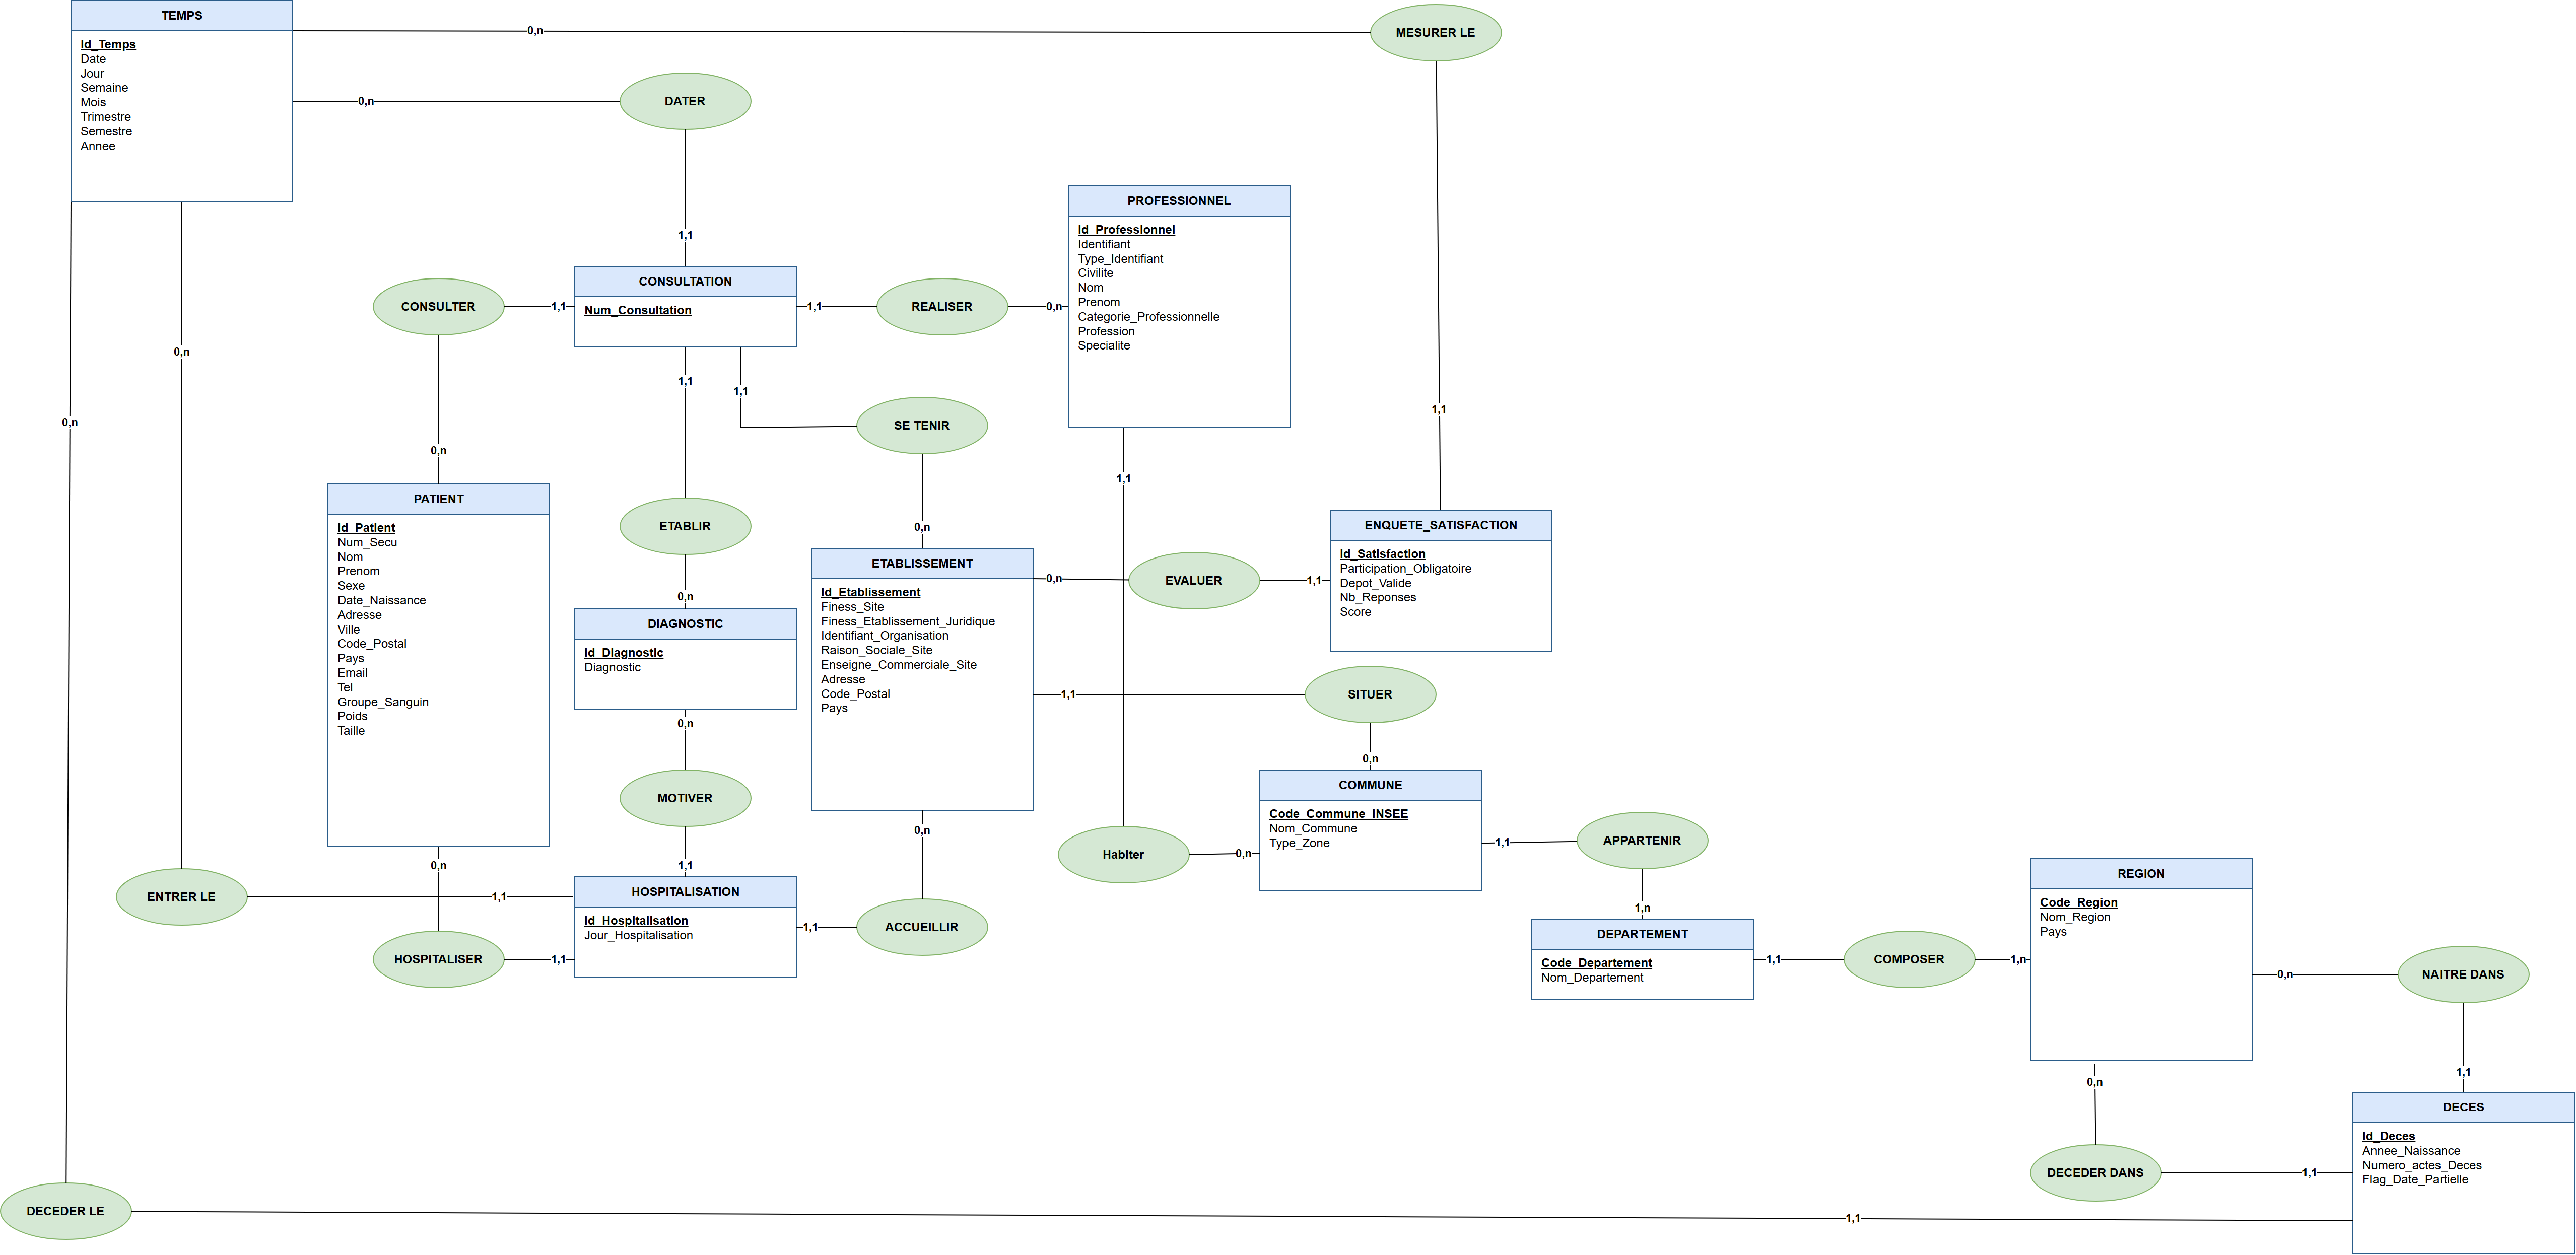
\includegraphics[width=\linewidth,height=0.62\textwidth,keepaspectratio]{contents/img/modele_conceptuel.png}
\end{center}

\newpage
\thispagestyle{fancy}
\subsection*{Annexe B -- Schéma logique en constellation}
\phantomsection
\addcontentsline{toc}{subsection}{Annexe B -- Schéma logique en constellation}

\noindent Constellation des quatre tables de faits et des six dimensions, avec leurs clés primaires (PK), étrangères (FK) et métier (BK). Ce schéma est décrit en partie~\ref{sec:logique}.

\begin{center}
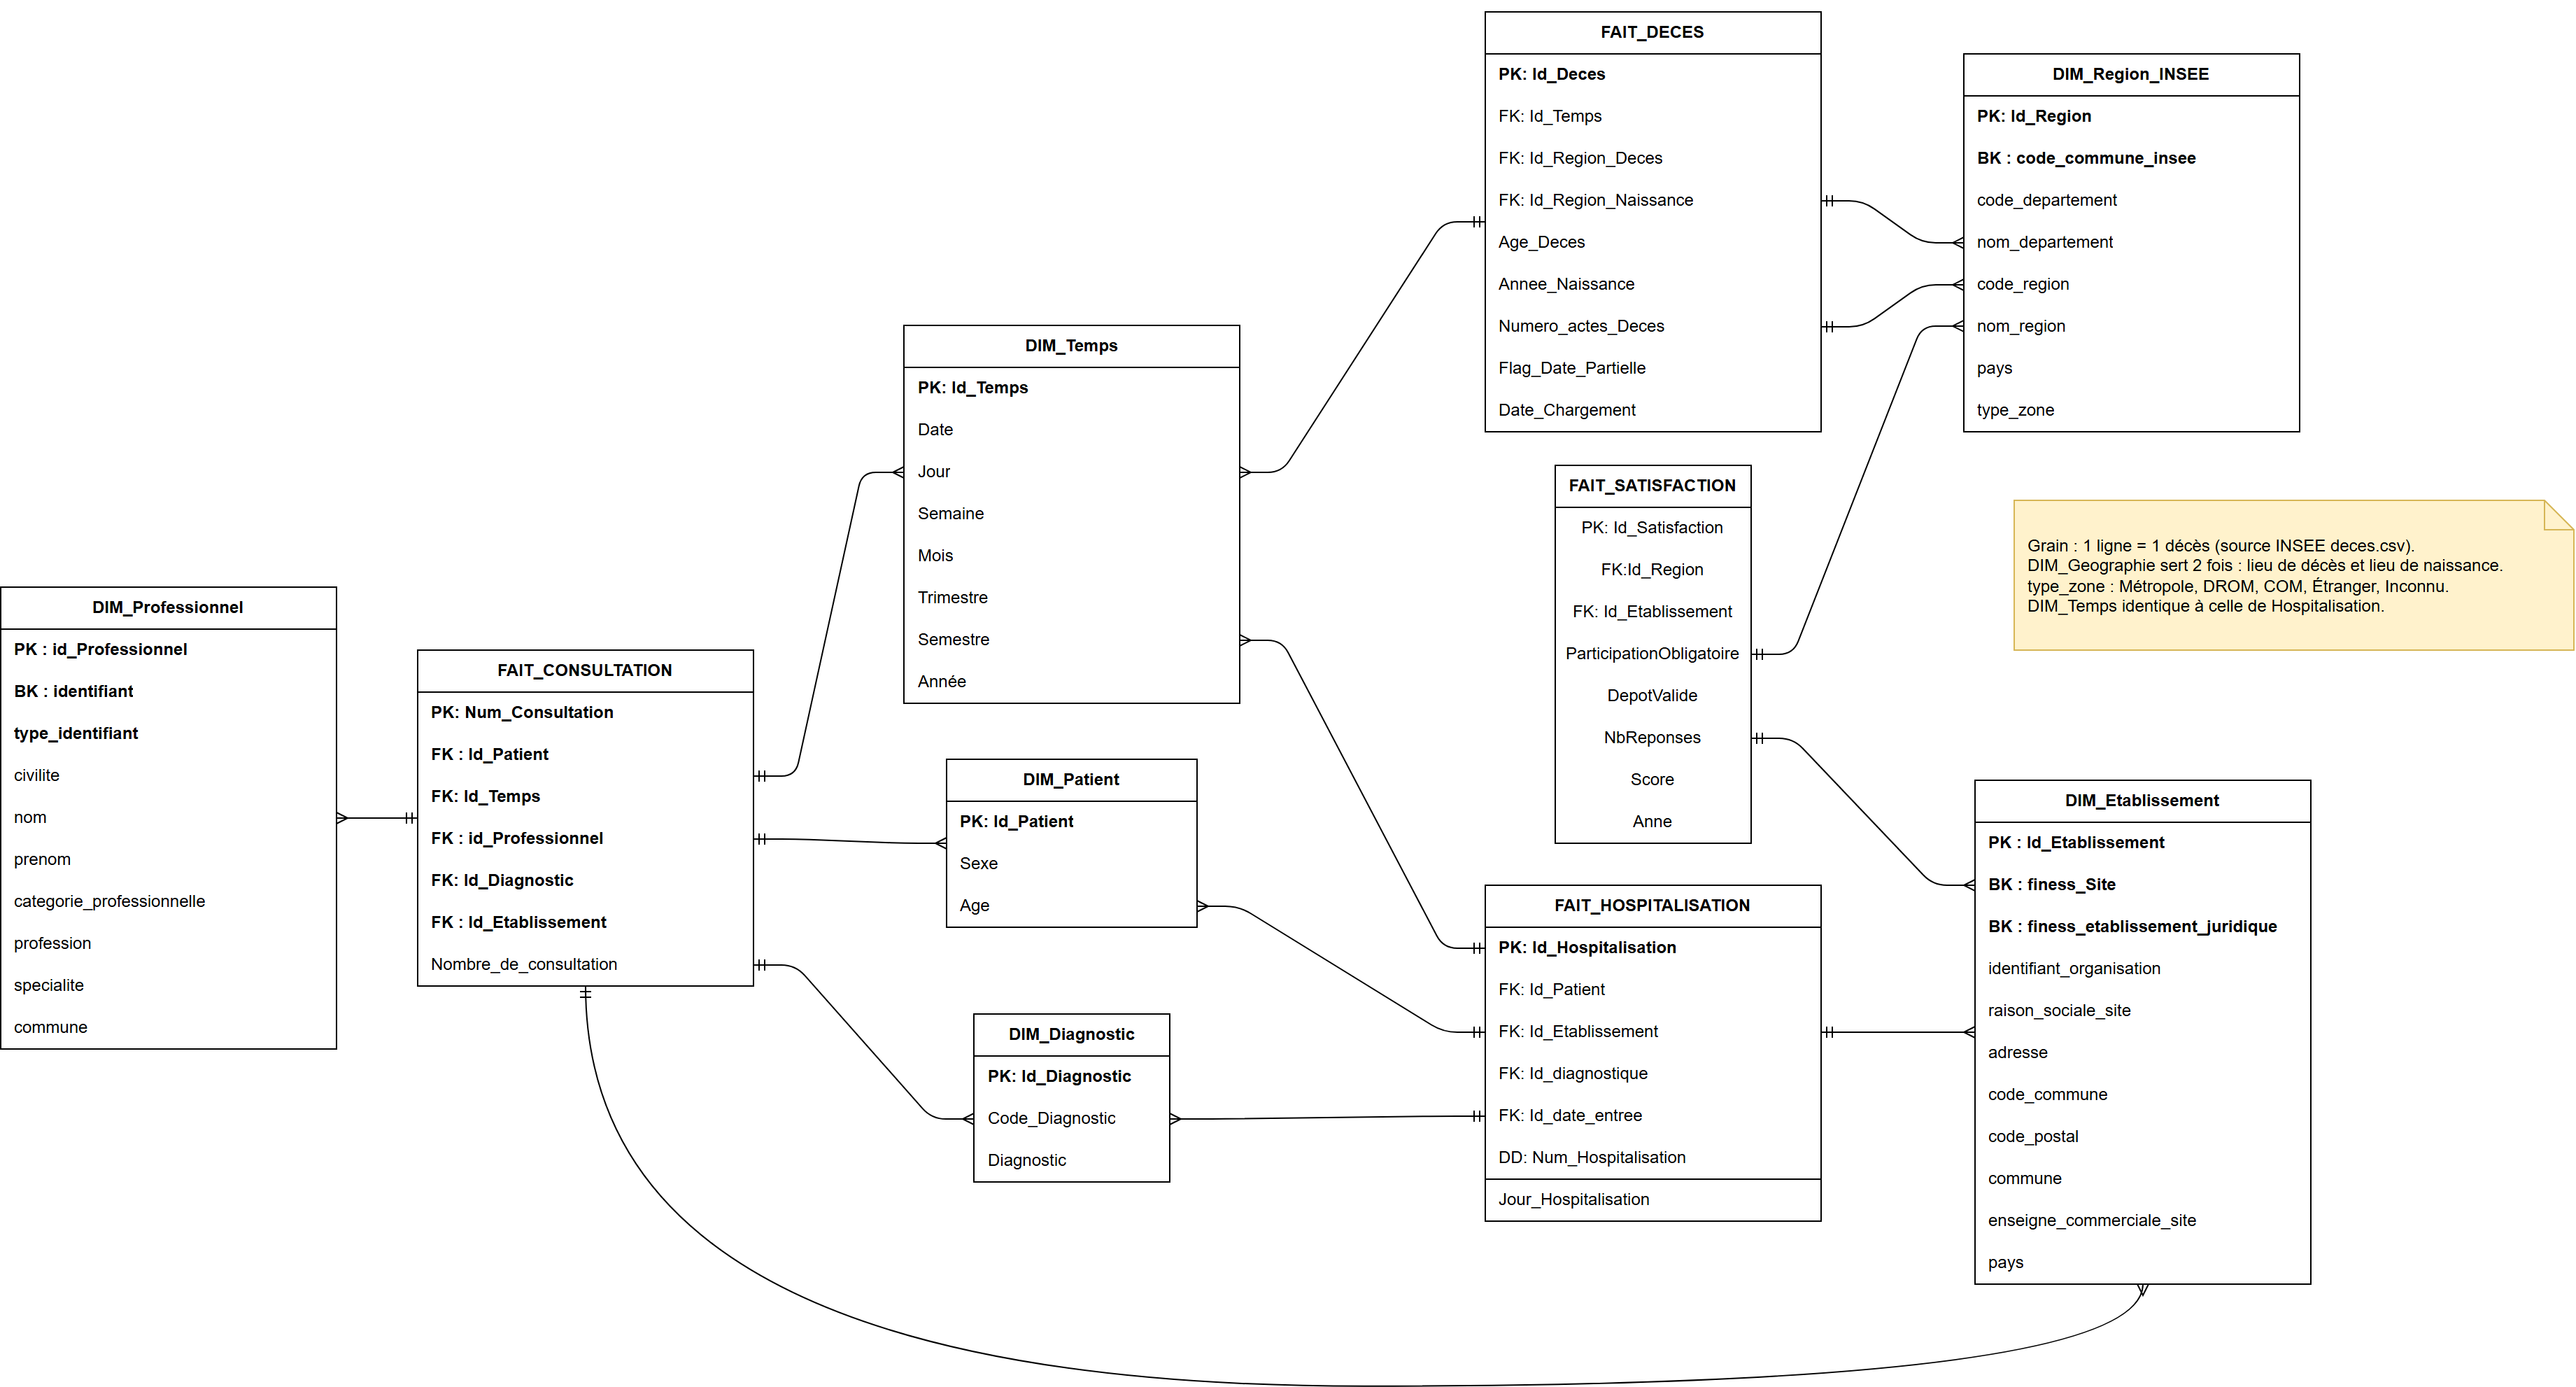
\includegraphics[width=\linewidth,height=0.62\textwidth,keepaspectratio]{contents/img/schema_constellation.png}
\end{center}
\end{landscape}


\end{document}
